\documentclass[italian,12pt,a4paper,oneside,final]{report}
\usepackage[toc]{appendix}
\usepackage{listings}
\usepackage{graphicx}
\usepackage{subcaption}
\usepackage[utf8]{inputenc}
\usepackage[T1]{fontenc}
\usepackage[backend=biber,style=numeric,sorting=none]{biblatex} %Imports biblatex package
\addbibresource{cnn2.bib} %Import the bibliography file
\usepackage[italian]{babel}
\usepackage[style=italian/quotes]{csquotes}
\usepackage{hyperref}
\graphicspath{ {images/} }
\lstset{
	captionpos=b,
	showspaces=false,
	basicstyle=\ttfamily,
	showstringspaces=false,
	breaklines=true,
	frame=line,
}
\renewcommand{\thesection}{\arabic{section}} % remove the \chapter counter from being printed with every \section
\renewcommand{\appendixtocname}{Appendice}
\renewcommand{\appendixpagename}{Appendice}
\hypersetup{
	colorlinks=true,
	citecolor=,
	linkcolor=,
	urlcolor=blue,
	pdftitle={Marco Giunta - Progetto ML},
	pdfauthor={Marco Giunta},
}


\title{\Large CNN2: Viewpoint Generalization via a Binocular Vision\\[0.5em]
\large Reproducibility Challenge}
\date{Luglio 2025}
\author{
Marco Giunta\thanks{Marco Giunta 147852 giunta.marco@spes.uniud.it}}


\begin{document}
\pagenumbering{roman}% To avoid duplicate hyperref links to pages with same page number
% Generate title page
\maketitle

% Generate TOCs
\pagenumbering{arabic}
\tableofcontents

\newpage
\section{Introduzione}

Lo scopo di questo progetto è riprodurre i risultati dell'articolo \citetitle{neurips2019:cnn2}\cite{neurips2019:cnn2} come proposto nella \citetitle{neurips2019:reproducibility-challenge}\cite{neurips2019:reproducibility-challenge}.
In particolare, l'obiettivo è quello di replicare i risultati principali presentati nell'articolo, senza utilizzare il codice rilasciato dagli autori, leggendo solo l'articolo e i materiali supplementari.

In questo progetto il modello è stato creato da zero usando la libreria PyTorch, anche se gli autori hanno messo a disposizione un repository\cite{cnn2:repository} su GitHub con il loro codice.

\subsection{Articolo originale}
Nell'articolo originale gli autori propongono il modello CNN\textsuperscript{2}, una rete neurale convoluzionale che riceve in input due immagini binoculari di un oggetto ed è in grado di riconoscere quell'oggetto da angolazioni diverse da quelle usate per l'addestramento del modello.

\subsubsection{Modello}
In figura~\ref{fig:cnn2_model} possiamo vedere l'architettura del modello CNN\textsuperscript{2}.
\begin{figure}[ht]
	\centering
	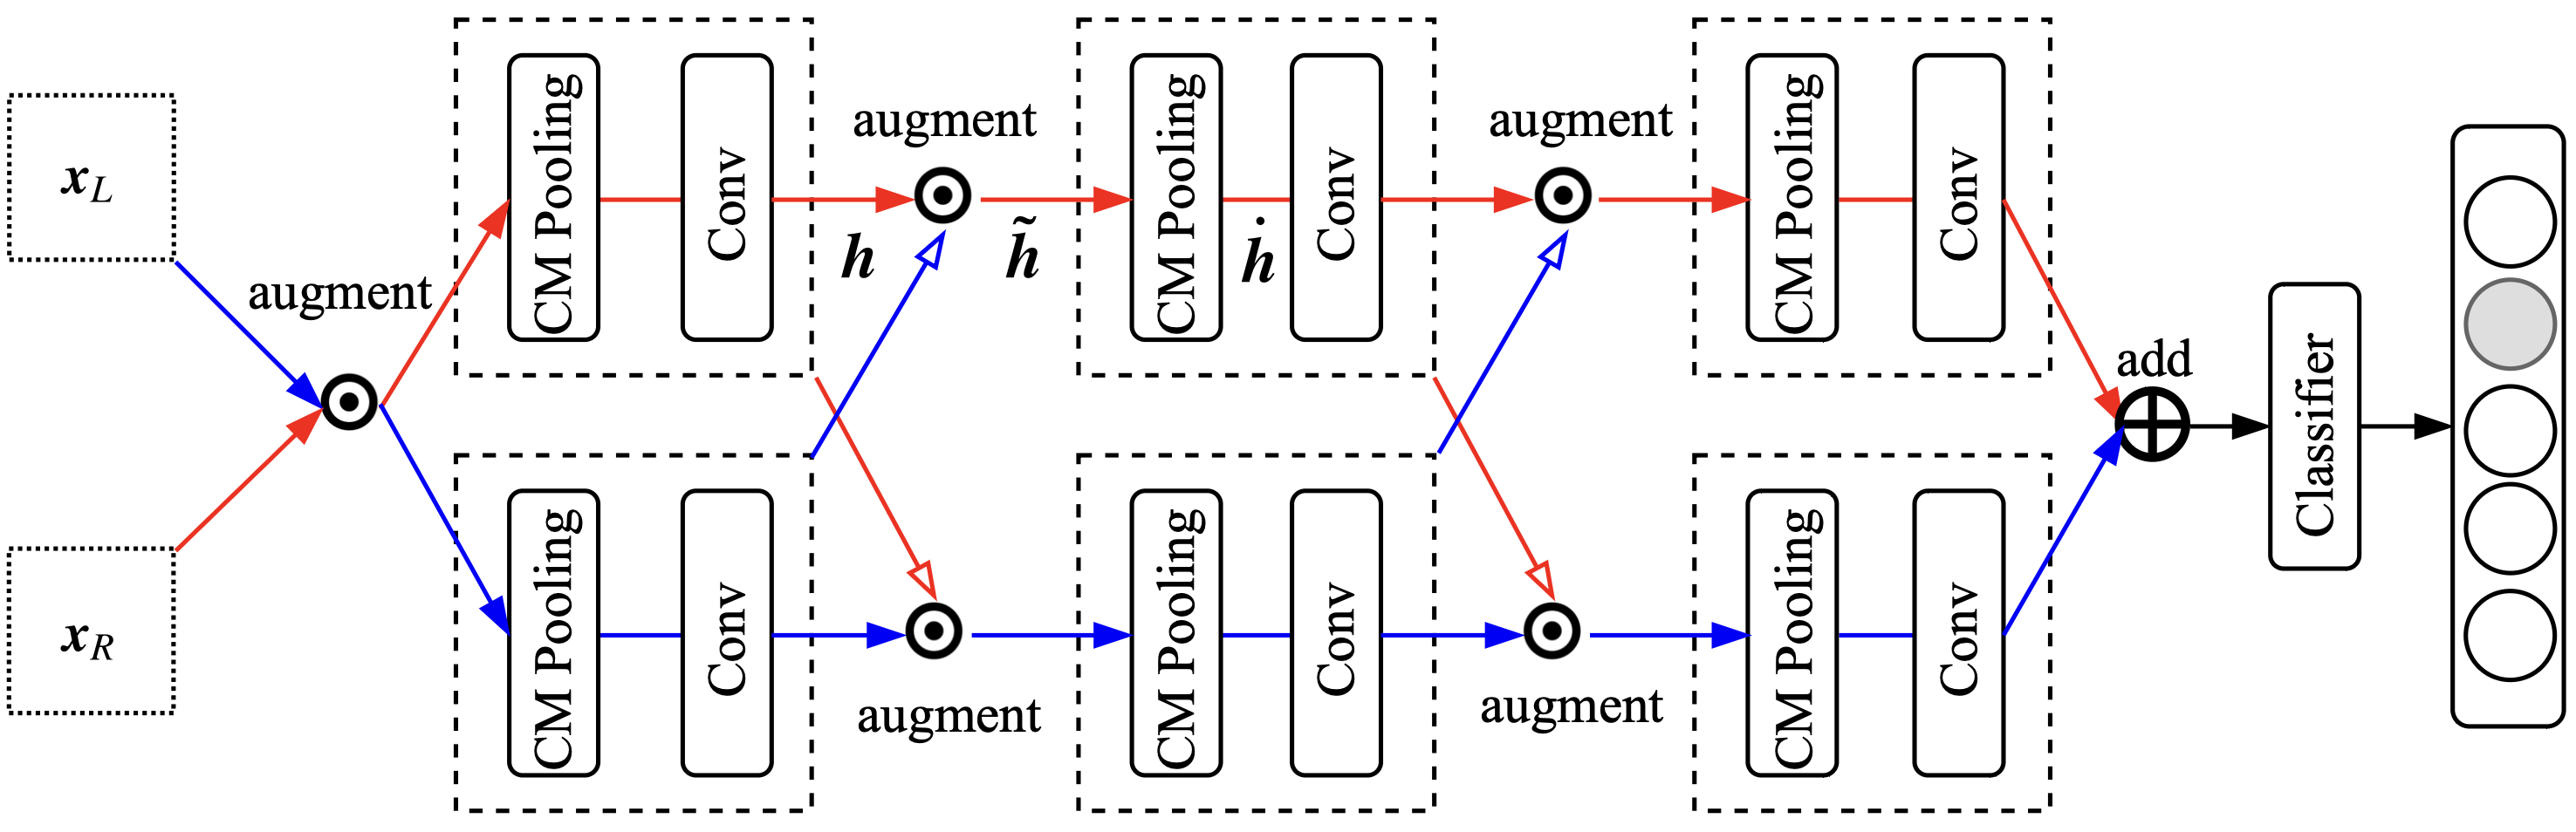
\includegraphics[width=1\textwidth]{model-cnn2.png}
	\caption{Modello CNN2}
	\label{fig:cnn2_model}
\end{figure}
A differenza di una CNN tradizionale, questo modello usa per le immagini dell'occhio sinistro e destro due percorsi di \textit{feedforward} paralleli ma complementari.
A ogni \textit{layer}, le immagini binoculari vengono combinate e poi suddivise seguendo la procedura di \textit{parallax augmentation} visibile in figura~\ref{fig:cnn2_parallax}.

Nello specifico, data una coppia di immagini binoculari, quella destra (\textit{h}\textsubscript{R}) viene combinata con \textit{h}\textsubscript{L} - \textit{h}\textsubscript{R}, mentre quella sinistra (\textit{h}\textsubscript{L}), con \textit{h}\textsubscript{R} - \textit{h}\textsubscript{L}: le due immagini \textit{aumentate} contengono le informazioni di entrambi gli occhi.
In figura~\ref{fig:smallnorb_augment_samples} vediamo un esempio di  \textit{parallax augmentation} di due immagini del dataset smallNORB.

\begin{figure}[ht]
	%\centerline{% center image to the page, not to text
		\centering
		\begin{subcaptionblock}{0.7\textwidth}
			\centering
			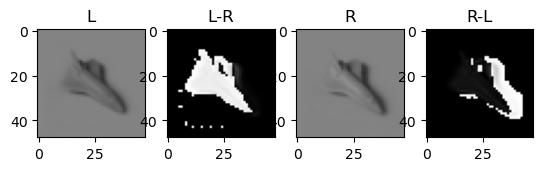
\includegraphics[width=1\linewidth]{smallnorb_augment_airplane.png}
			\caption{Aeroplano}
			\label{fig:smallnorb_augment_airplane}
		\end{subcaptionblock}%
		\hfill
		\begin{subcaptionblock}{0.7\textwidth}
			\centering
			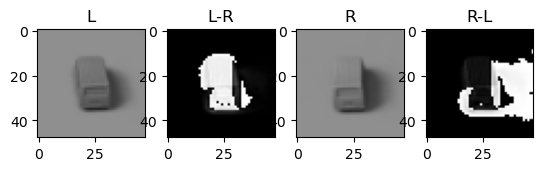
\includegraphics[width=1\linewidth]{smallnorb_augment_truck.png}
			\caption{Camion}
			\label{fig:smallnorb_augment_truck}
		\end{subcaptionblock}%
		%}
	\caption{Esempi di parallax augmentation del dataset smallNORB}
	\label{fig:smallnorb_augment_samples}
\end{figure}

\noindent Ciascuna mappa aumentata viene immessa nel livello successivo attraverso il percorso sinistro o destro.
Questo consente ai filtri nei livelli convoluzionali di rilevare le caratteristiche stereoscopiche, osservando la parallasse e confrontando le parti nitide e sfocate.
\begin{figure}[!ht]
	\centering
	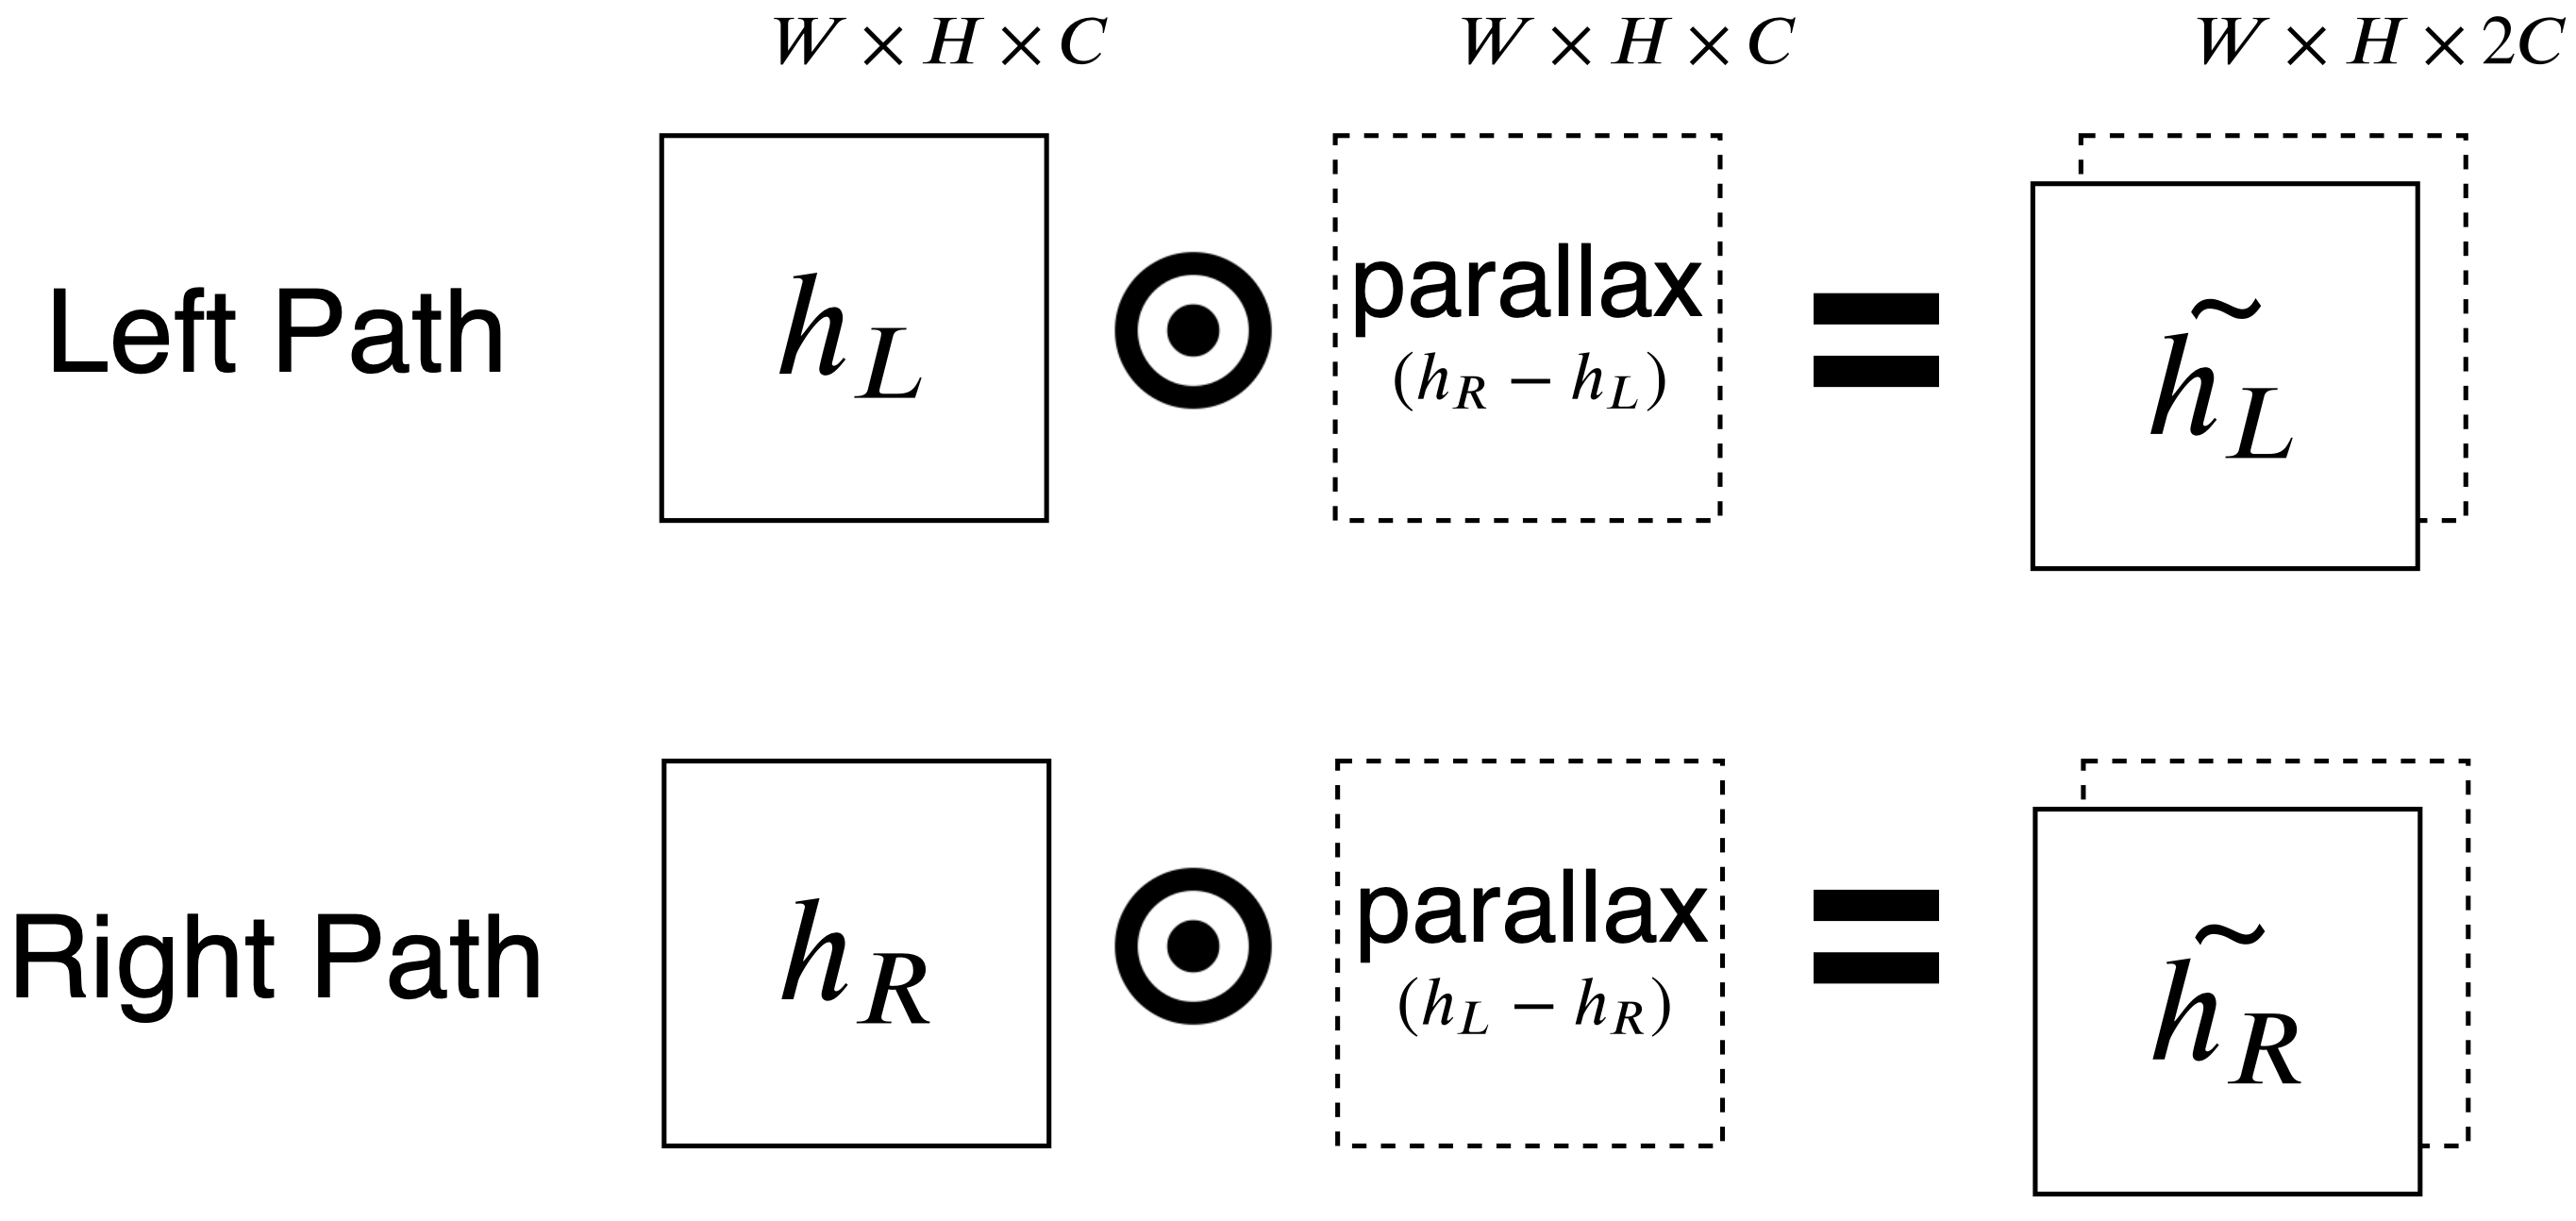
\includegraphics[width=0.8\textwidth]{parallax.png}
	\caption{Parallax augmentation}
	\label{fig:cnn2_parallax}
\end{figure}

\noindent Oltre alla \textit{parallax augmentation}, gli autori hanno introdotto un nuovo tipo di livello di \textit{pooling}, chiamato \textit{concentric multi-scale (CM) pooling}.
La figura~\ref{fig:cnn2_cmpooling} mostra come funziona il pooling CM: data un'immagine aumentata si ottengono delle mappe temporanee, alla quali si applica un operazione di \textit{max pooling }, per poi sovrapporsi lungo la dimensione del canale del tensore di input.
\begin{figure}[ht]
	\centering
	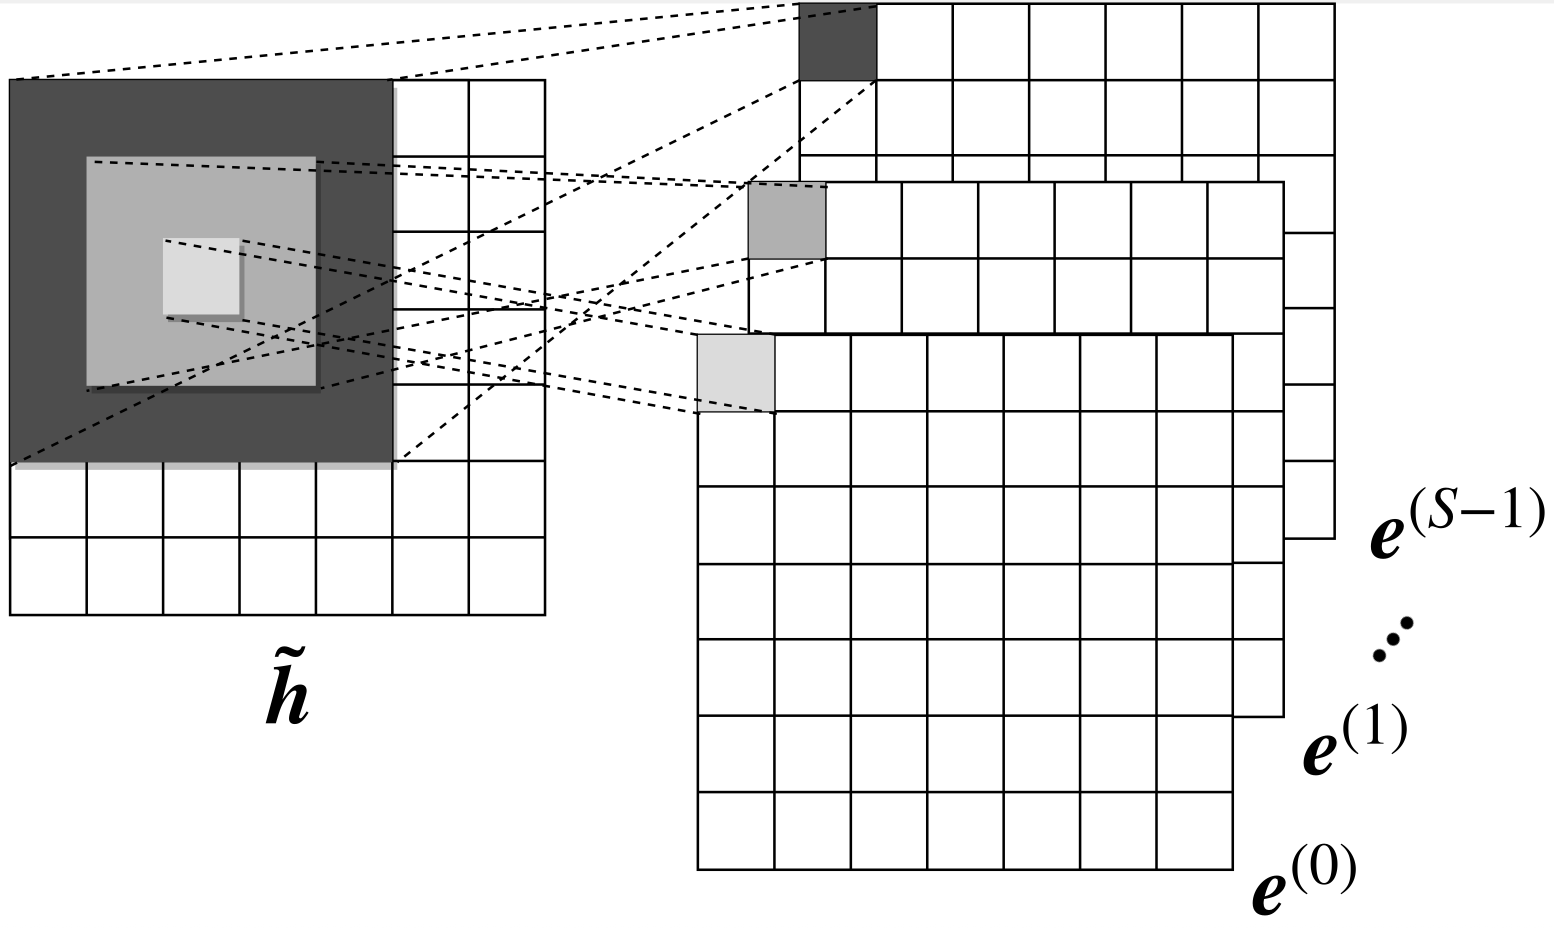
\includegraphics[width=0.8\textwidth]{cmpooling.png}
	\caption{CM Pooling}
	\label{fig:cnn2_cmpooling}
\end{figure}

\noindent A differenza dei livelli di pooling convenzionali che seguono i livelli convoluzionali, i livelli di pooling CM vengono posizionati prima di questi e non modificano la larghezza e l'altezza dell'immagine di input.
Questo aiuta il filtro nel livello successivo a rilevare facilmente i pattern stereoscopici, contrastando le caratteristiche sfocate dello sfondo con quelle nitide in primo piano.
In figura~\ref{fig:smallnorb_cmpooling_samples} vediamo un esempio di cosa succede alla fine del primo livello di CM a due immagini del dataset smallNORB. 

\begin{figure}[!ht]
	%\centerline{% center image to the page, not to text
		\centering
		\begin{subcaptionblock}{0.7\textwidth}
			\centering
			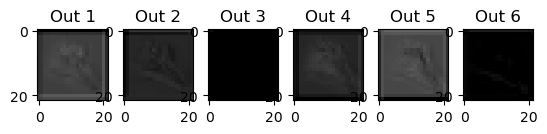
\includegraphics[width=1\linewidth]{smallnorb_M1_out_airplane.png}
			\caption{Aeroplano}
			\label{fig:smallnorb_M1_out_airplane}
		\end{subcaptionblock}%
		\hfill
		\begin{subcaptionblock}{0.7\textwidth}
			\centering
			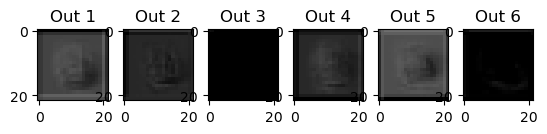
\includegraphics[width=1\linewidth]{smallnorb_M1_out_truck.png}
			\caption{Camion}
			\label{fig:smallnorb_M1_out_truck}
		\end{subcaptionblock}%
	%}
	\caption{Esempi di parallax augmentation del dataset smallNORB}
	\label{fig:smallnorb_cmpooling_samples}
\end{figure}

\subsubsection{Parametri}
All'interno dell'articolo\cite{neurips2019:cnn2} e del materiale supplementare\cite{cnn2:supplementary} gli autori hanno descritto parte della struttura del modello e i parametri utilizzati per realizzarla.

\begin{foreigndisplaycquote}{english}[\S3.2]{cnn2:supplementary}
We train each model using Adam algorithm ($\ldots$) with mini-batches of size 32.
We use early stopping strategy for all experiments.\\
$\ldots$\\
Our CNN\textsuperscript{2} consists of 3 blocks. Each block has a CM pooling layer and a convolution layer.
We use 3 scales (s = 0, 1, 2) in a CM pooling layer.
The first, second, and third convolution layers have 6, 12, and 32 filters with sizes 5 x 5, 5 × 5, and 3 x 3 respectively.
All filters use the stride of 1, and each unit uses the ReLU non-linearity.
\end{foreigndisplaycquote}
Purtroppo non hanno inserito nessun dettaglio relativo al classificatore presente in figura~\ref{fig:cnn2_model} e non ci sono informazioni ne sulla configurazione dell'\textit{early stopping} ne sulla presenza o meno di un layer di \textit{dropout}.

Fortunatamente gli autori hanno rilasciato il codice\cite{cnn2:repository} Python del modello, realizzato usando la libreria TensorFlow: in questo modo sono state ricavate le informazioni relative al classificatore e al layer di \textit{dropout}.
Non è stato possibile invece ricavare la configurazione dell'\textit{early stopping}, visto che non era presente nemmeno del codice.

\section{Dataset}
Nel paper originale gli autori hanno utilizzato per il loro modello tre diversi dataset: vediamoli in dettaglio.

Only the SmallNORB dataset provides binocular images.
For the rest of the datasets, we use pairs of images having successive azimuths degrees to simulate
binocular images. We also sample 5 classes of objects from each dataset that look different from each
other in any azimuths degree. 


\subsection{small NORB}
Questo dataset\cite{dataset:smallnorb}, destinato a esperimenti per il riconoscimento di oggetti 3D dalla loro forma, è composto da 48.600 immagini binoculari in scala di grigi di 50 giocattoli appartenenti a 5 diverse categorie.

\noindent Le categorie sono:
\begin{itemize}
	\item animali a 4 zampe
	\item figure umane
	\item aeroplani
	\item camion
	\item automobili
\end{itemize}
Ogni immagine binoculare è una coppia di file di grandezza 96x96 pixels.
Gli oggetti sono stati fotografati da una coppia di telecamere sotto 6 diverse condizioni di luce, 9 angolazioni (da 30 a 60 gradi, con passo 5 gradi) e 18 \textit{azimuths} (da 0 a 340 gradi con passo 20 gradi).
Il training set è composto da 5 istanze di ogni categoria (la 4, 6, 7, 8 e 9) e il test set dalle restanti (0, 1, 2, 3, e 5): ogni istanza ha 972 immagini binoculari.
In figura ~\ref{fig:smallnorb_samples} possiamo vedere alcuni esempi di immagini del dataset.
\begin{figure}[!ht]
	\centerline{% center image to the page, not to text
		\begin{subcaptionblock}{0.4\textwidth}
			\centering
			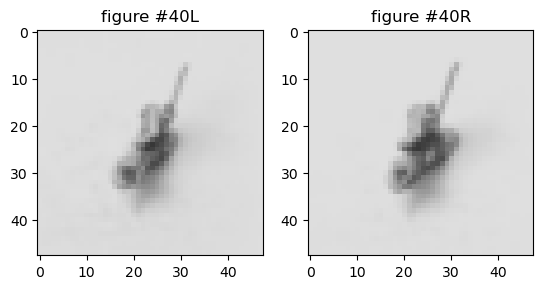
\includegraphics[width=1\linewidth]{smallnorb_figure.png}
			\caption{Figura umana}
			\label{fig:smallnorb_figure}
		\end{subcaptionblock}%
		\begin{subcaptionblock}{0.4\textwidth}
			\centering
			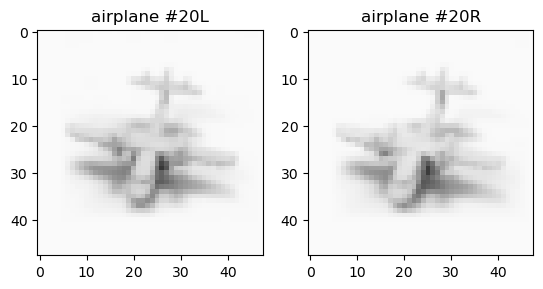
\includegraphics[width=1\linewidth]{smallnorb_airplane.png}
			\caption{Aeroplano}
			\label{fig:smallnorb_airplane}
		\end{subcaptionblock}%
		\begin{subcaptionblock}{0.4\textwidth}
			\centering
			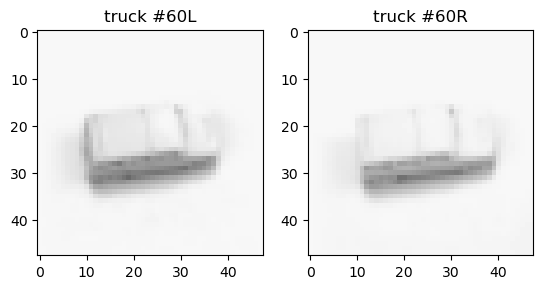
\includegraphics[width=1\linewidth]{smallnorb_truck.png}
			\caption{Camion}
			\label{fig:smallnorb_truck}
		\end{subcaptionblock}%
	}
	\caption{Esempi di immagini del dataset smallNORB}
	\label{fig:smallnorb_samples}
\end{figure}

\subsection{ModelNet2D}
%TODO ModelNet40
Il dataset ModelNet40\cite{dataset:modelnet40} contiene circa 12.311 modelli CAD suddivisi in 40 classi.
Gli autori hanno selezionato 5 classi:
\begin{itemize}
	\item sedie
	\item figure umane
	\item aeroplani
	\item automobili
	\item lampade
\end{itemize}
e, per ciascuna classe, hanno preso 15 oggetti a caso.
Per ogni oggetto è stato fatto il render con 72 angoli di azimuth (con passo di 5 gradi), 9 angolazioni (da 30 a 70 gradi, con passo 5 gradi) sotto condizioni di luce fisse, per un totale di 648 immagini in scala di grigio con risoluzione 96x96 pixel.
Seguendo questi passaggi, hanno ottenuto 48.600 immagini: questo subset è stato chiamato dagli autori ModelNet2D.
In figura ~\ref{fig:modelnet2d_samples} possiamo vedere alcuni esempi di immagini del dataset.
\begin{figure}[!ht]
	\centerline{% center image to the page, not to text
		\begin{subcaptionblock}{0.4\textwidth}
			\centering
			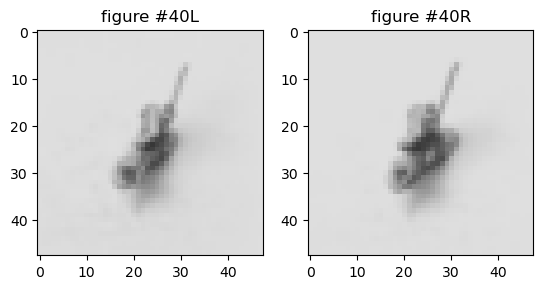
\includegraphics[width=1\linewidth]{smallnorb_figure.png}
			\caption{Figura umana}
			\label{fig:modelnet2d_figure}
		\end{subcaptionblock}%
		\begin{subcaptionblock}{0.4\textwidth}
			\centering
			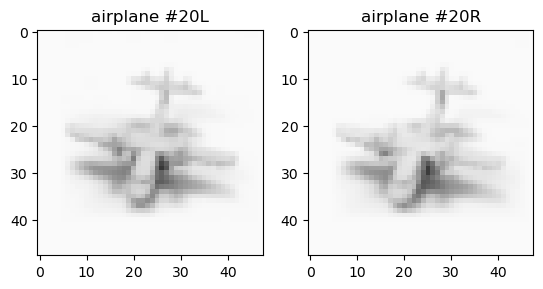
\includegraphics[width=1\linewidth]{smallnorb_airplane.png}
			\caption{Aeroplano}
			\label{fig:modelnet2db_airplane}
		\end{subcaptionblock}%
		\begin{subcaptionblock}{0.4\textwidth}
			\centering
			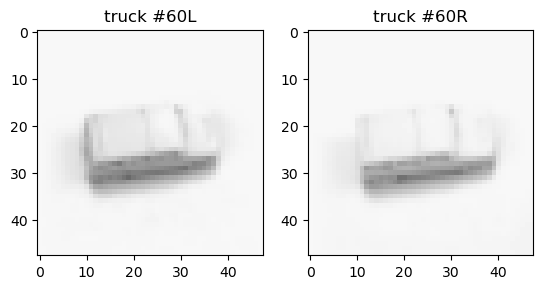
\includegraphics[width=1\linewidth]{smallnorb_truck.png}
			\caption{Camion}
			\label{fig:modelnet2d_truck}
		\end{subcaptionblock}%
	}
	\caption{Esempi di immagini del dataset ModelNet2d}
	\label{fig:modelnet2d_samples}
\end{figure}

\subsection{RGB-D Object}
%TODO RGB-D Object
Questo dataset\cite{dataset:rgb-d},
This dataset includes 300 common household objects in 51
classes. It was recorded using a Kinect style 3D camera that records synchronized and aligned
640x480 RGB and depth images. Each object was placed on a turntable and video sequences were
captured for one whole rotation. For each object, there are 3 video sequences, each recorded with
the camera mounted at a different height so that the object is viewed from different angles with the
horizon. We take images of the same object with angles at multiples of 10 degrees and get 250,000
colored images in total.

“camera,” “flashlight,” “lightbulb,” “pitcher,” and “stapler”

A Large-Scale Hierarchical Multi-View RGB-D Object Dataset 
Kevin Lai, Liefeng Bo, Xiaofeng Ren, and Dieter Fox 
IEEE International Conference on Robotics and Automation (ICRA), May 2011.

\section{Risultati ottenuti}

\subsection{small NORB}

\subsubsection{Codice originale}
Il codice originale presente nel repository degli autori differisce da quanto scritto nell'articolo: in particolare, la divisione del dataset non è la stessa.
Nell'articolo viene definita in questo modo:

\begin{foreigndisplaycquote}{english}[\S4.1]{neurips2019:cnn2}
On the SmallNORB dataset, we use the images taken from azimuths of degrees from 20 to 80 as the training set, degrees at 0 and 100 as the validation set, and the rest as the test set.
\end{foreigndisplaycquote}
mentre nel codice, il training set è pari a \(\frac{1}{3}\) di tutte le immagini (16200) e il test set è composto da tutto il resto (32400).
Nel codice manca completamente il validation set.
\begin{table}[!ht]
	\centering
	\begin{tabular}[t]{|c|cc|}
		\hline
		& \textbf{Accuracy} & \textbf{Loss} \\
		\hline
		training set codice autori& 0.888 & 1.727 \\
		training set articolo& 0.775 & 6.631 \\
		training set maggiore& 0.958 & 0.397 \\
		articolo & 0.865 & - \\ 
		\hline
	\end{tabular}
	\caption{Test loss/accuracy smallNORB (con validation set)}
	\label{tab:smallnorb_val_loss_acc}
\end{table}

\noindent Utilizzando la suddivisione del dataset presente nel codice (training set: 16200, test set: 32400), il risultato è quello nella prima riga della tabella~\ref{tab:smallnorb_val_loss_acc}, abbastanza in linea con quanto scritto nell'articolo.
Invece, modificando il codice originale (per suddividere il dataset come descritto nell'articolo, cioè training set: 10800, validation set: 5400 e test set: 32400), il risultato cambia, come si può vedere nella seconda riga della tabella~\ref{tab:smallnorb_val_loss_acc}: in entrambi i casi è presente un valore di loss molto elevato.
In figura~\ref{fig:smallnorb_train_val_loss_acc_original} possiamo osservare che, usando la suddivisione del dataset indicata nell'articolo, la validation loss ha una curva anomala.

\begin{figure}[ht]
	\centerline{% center image to the page, not to text
	\begin{subcaptionblock}{0.6\textwidth}
		\centering
		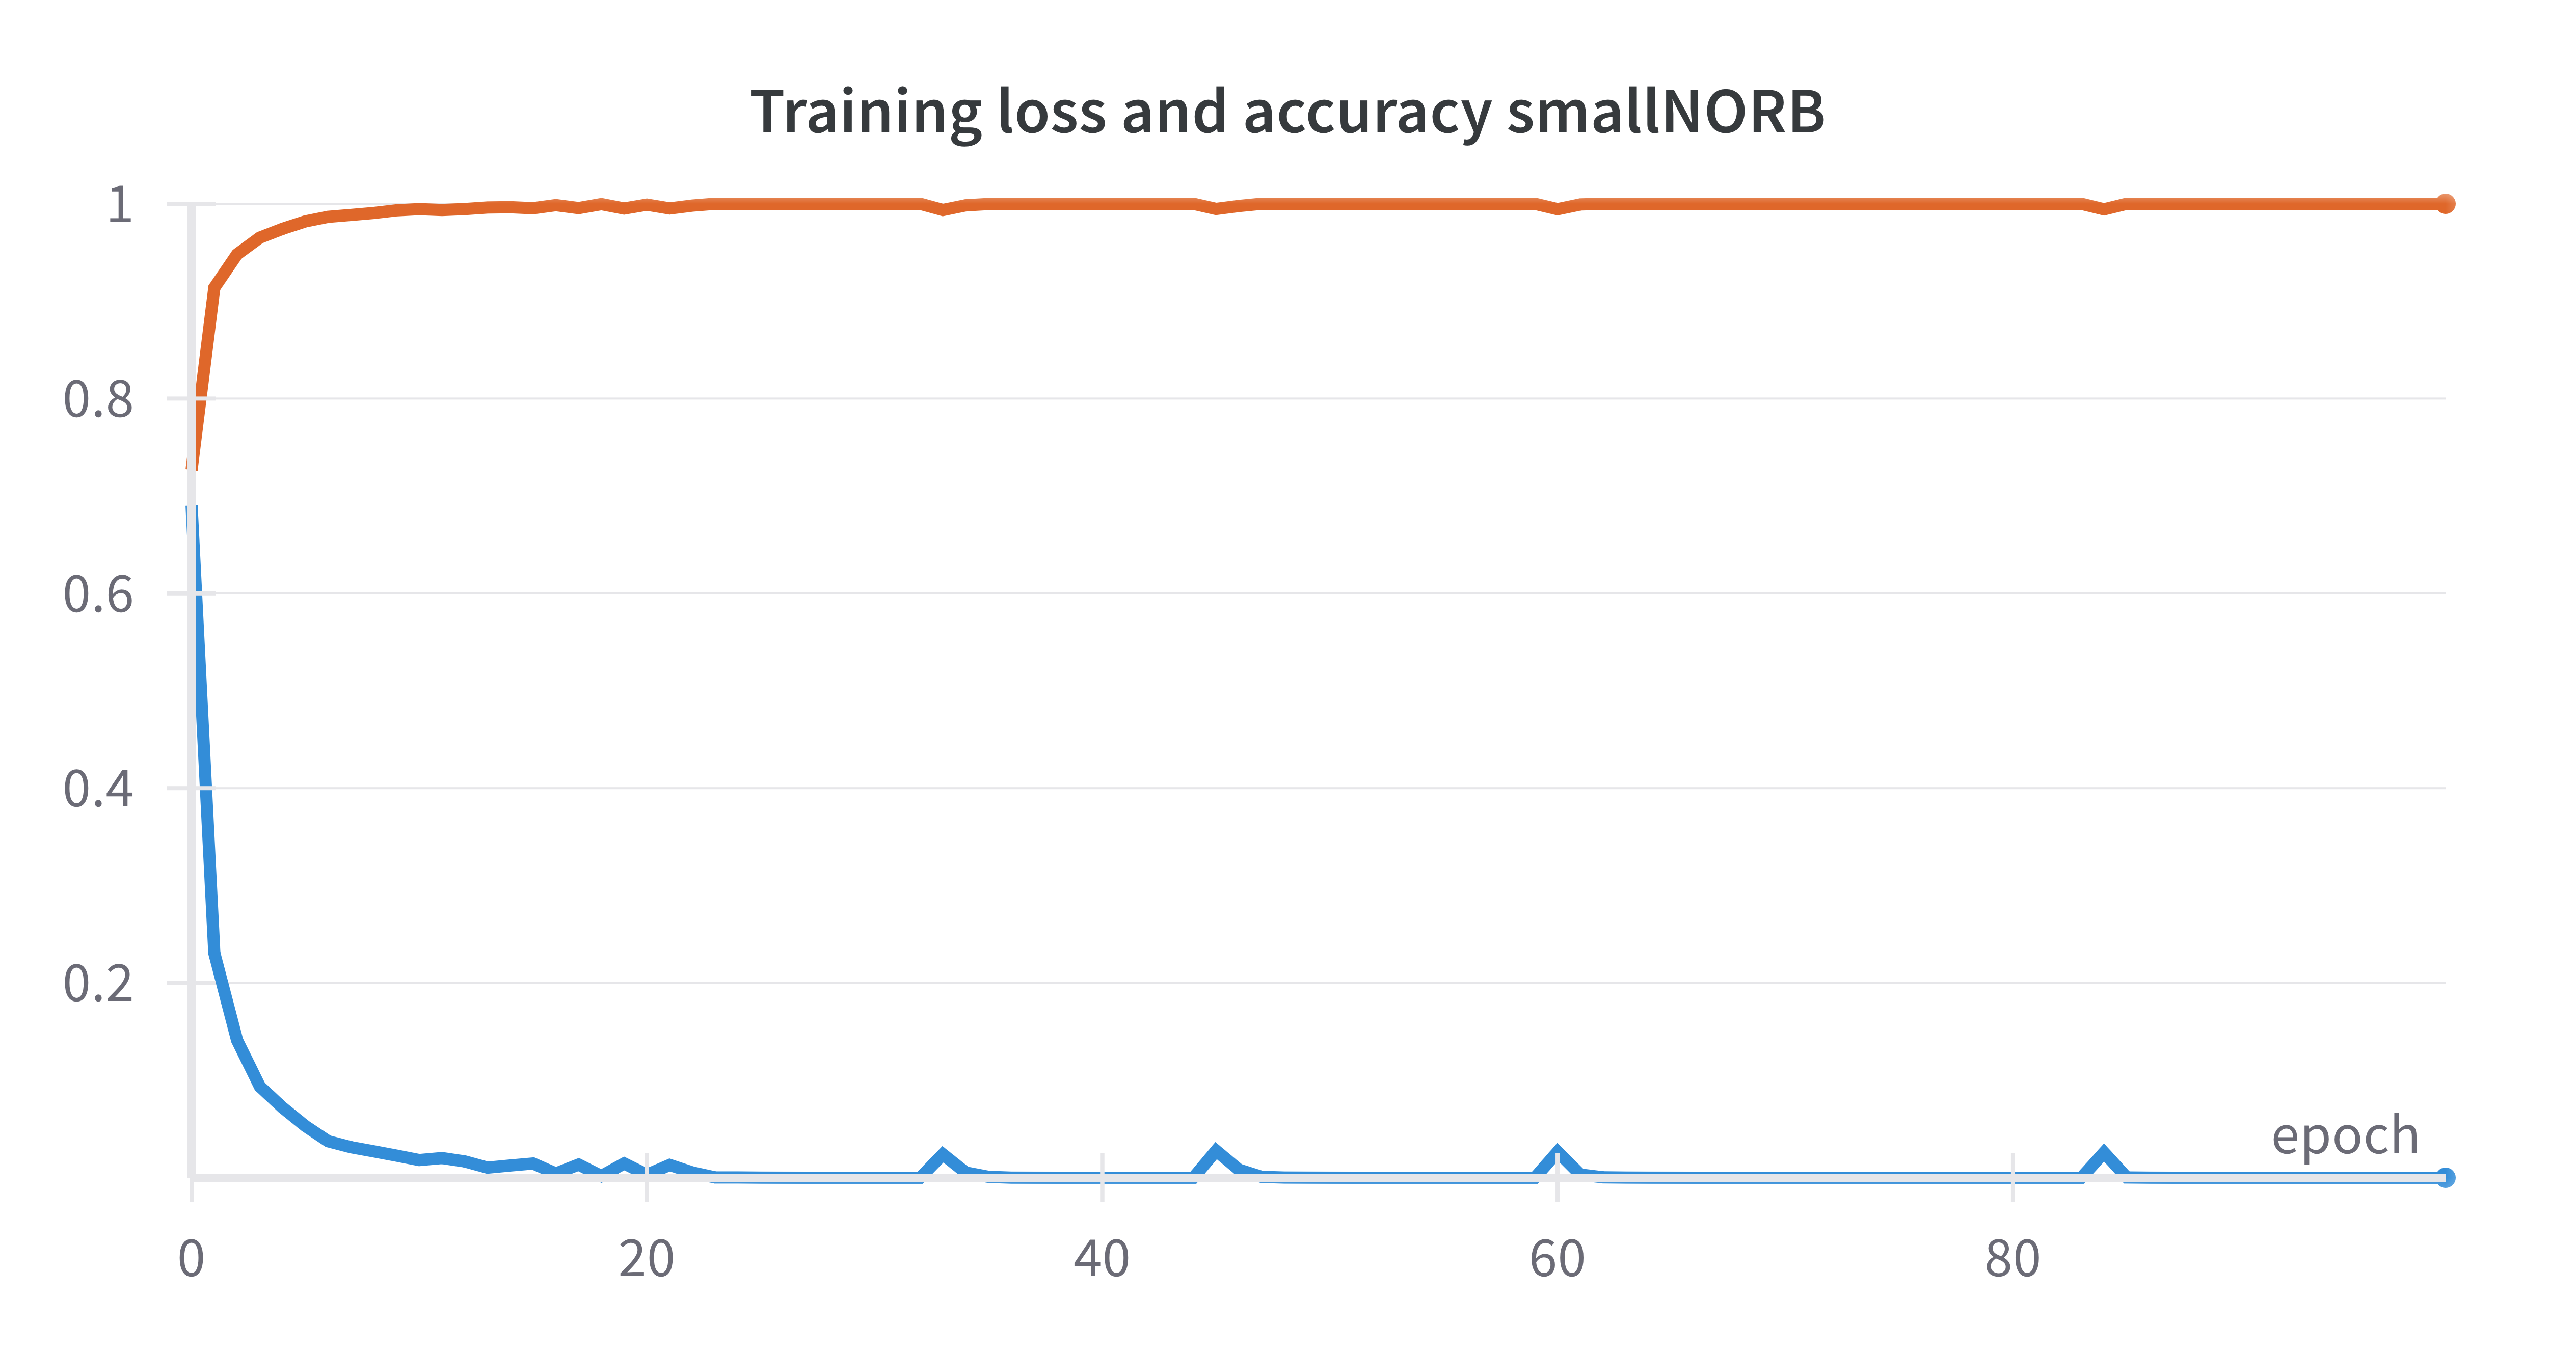
\includegraphics[width=1\linewidth]{smallnorb_train_loss_acc_original.png}
		\caption{Training  loss/accuracy}
		\label{fig:smallnorb_train_loss_acc_original}
	\end{subcaptionblock}%
	\begin{subcaptionblock}{0.6\textwidth}
		\centering
		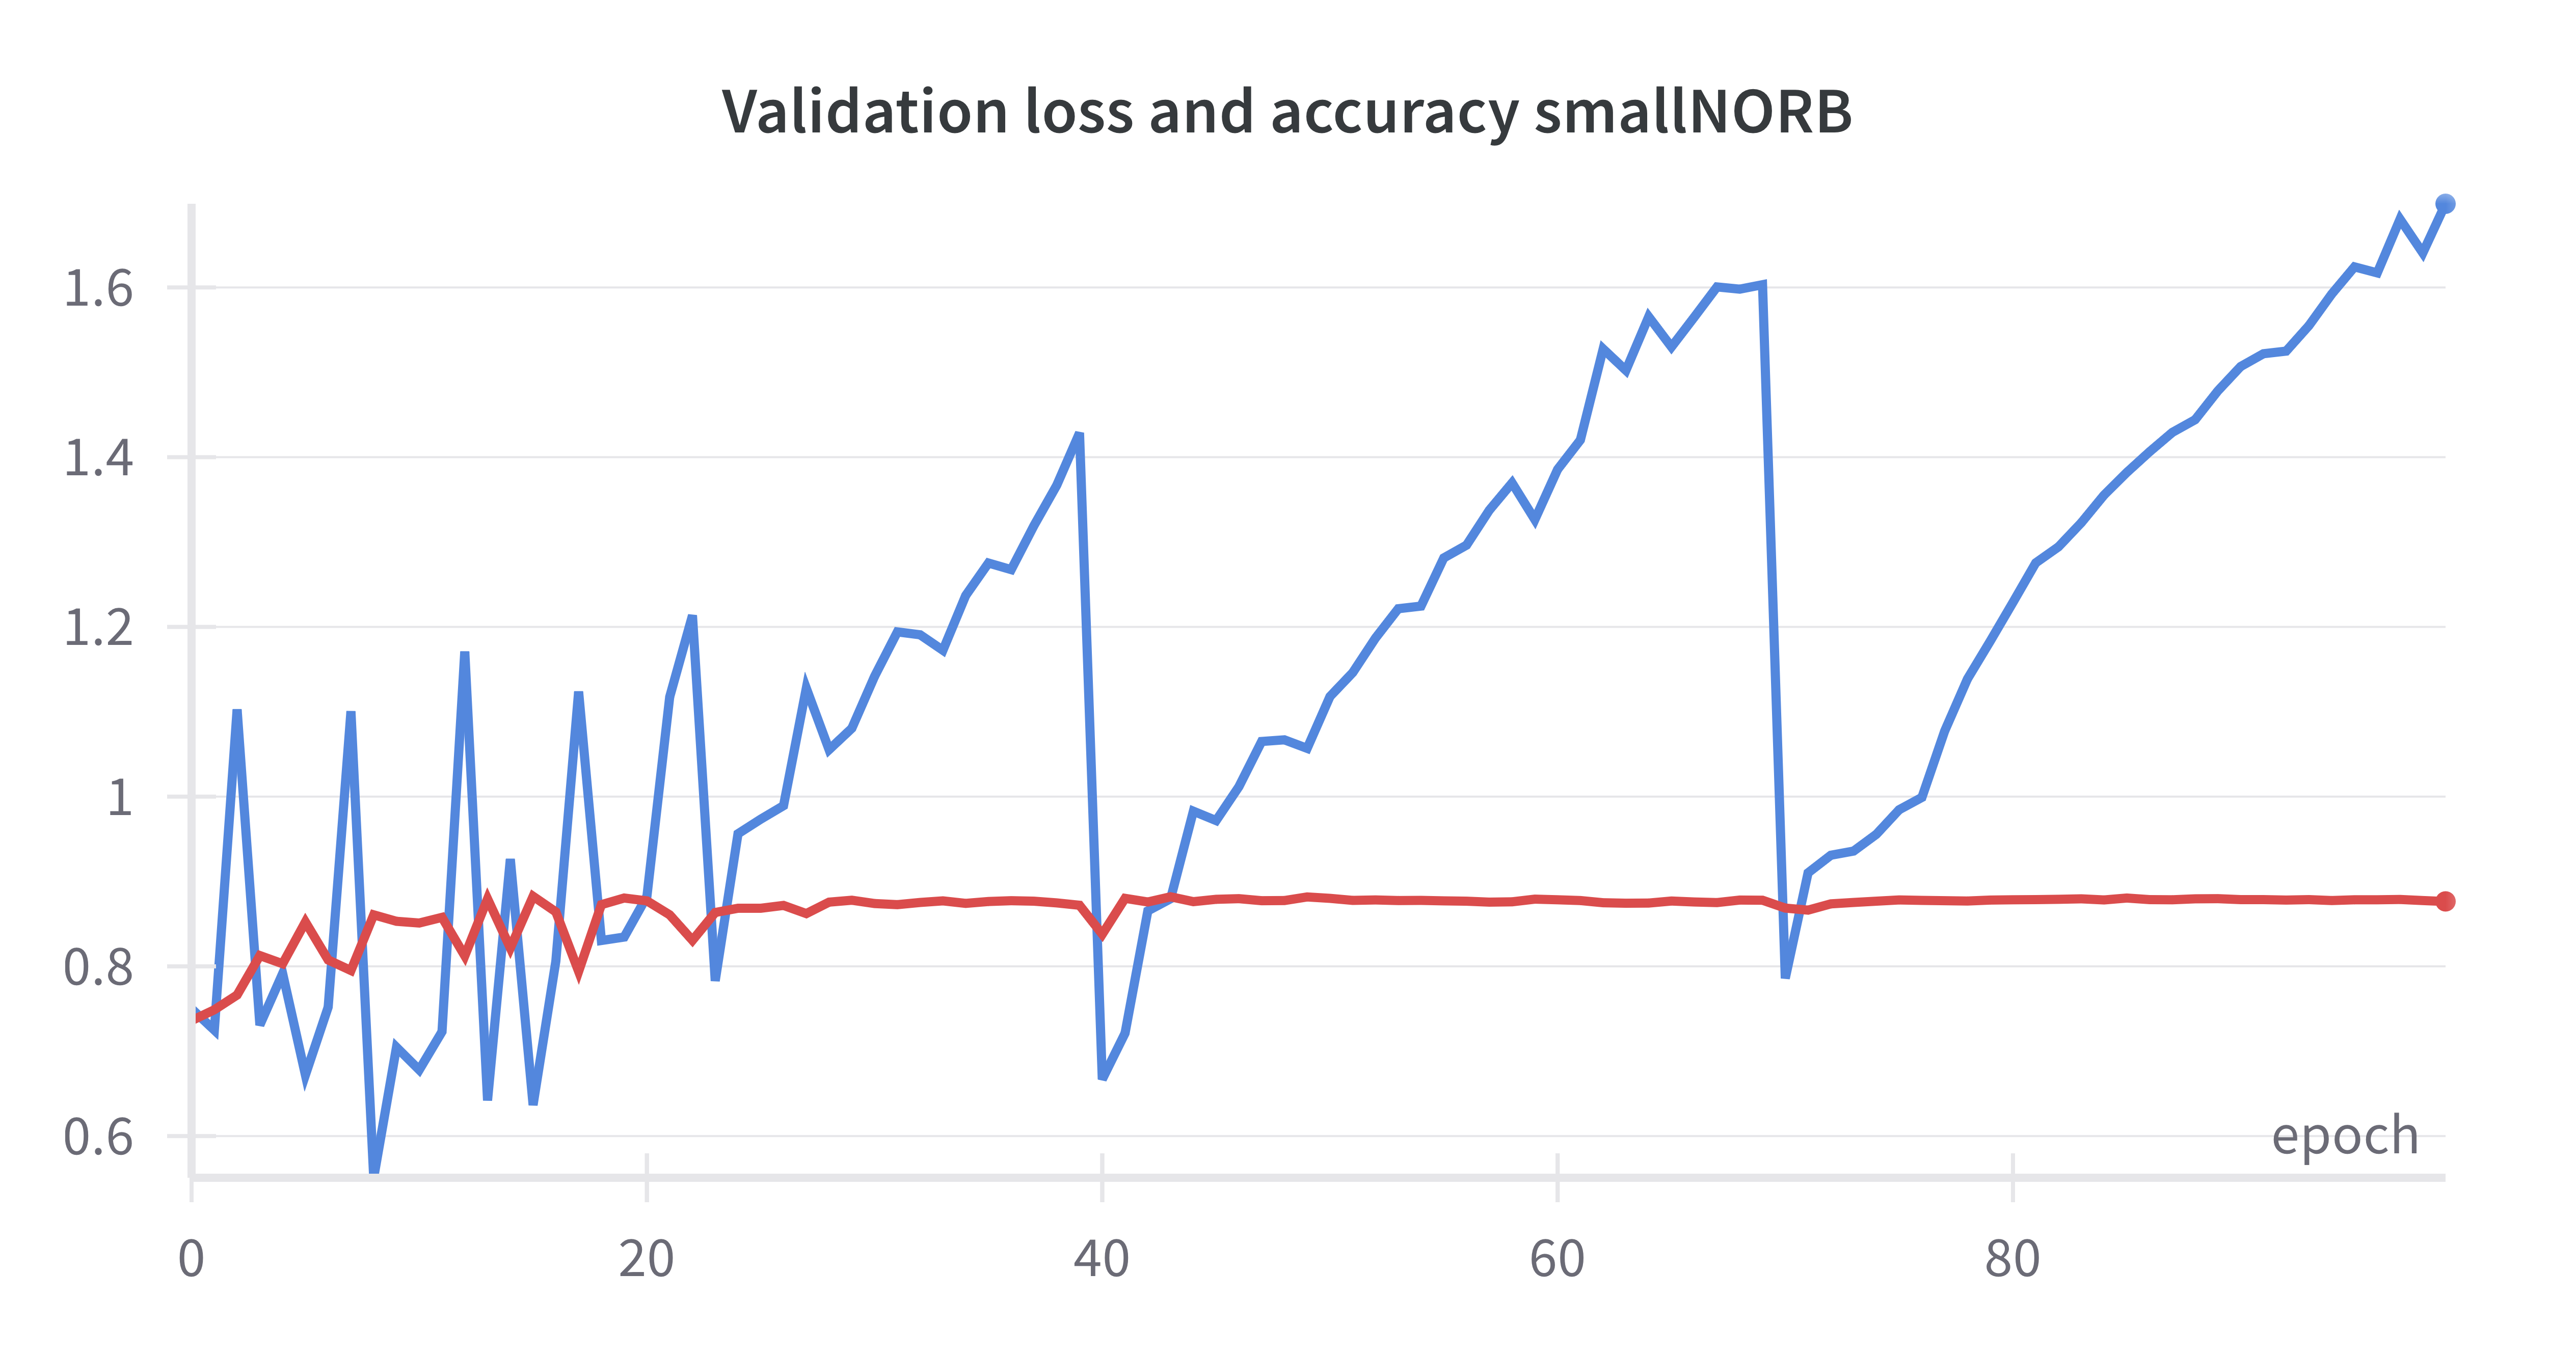
\includegraphics[width=1\linewidth]{smallnorb_val_loss_acc_original.png}
		\caption{Validation loss/accuracy}
		\label{fig:smallnorb_val_loss_acc_original}
	\end{subcaptionblock}%
	}
	\caption{Metriche del dataset smallNORB (con validation set)}
	\label{fig:smallnorb_train_val_loss_acc_original}
\end{figure}
Di solito, un valore di accuracy che aumenta e quello di loss che non tente a diminiuire, indica che il modello è in \textit{over-fitting}, cioè è in grado di memorizzare i pattern del training data e non riesce a funzionare bene con altri dati.
Un modo per risolvere questo problema è aumentare il numero di dati del training set.
Modificando il codice originale, aumentando i dati del training set a 21600 e riducendo quelli del test set a 21600, il modello sembra funzionare meglio, come possiamo vedere in figura~\ref{fig:smallnorb_train_val_loss_acc_mod}.
I risultati ottenuti sono quelli presenti nella terza riga della tabella~\ref{tab:smallnorb_val_loss_acc}.

\begin{figure}[ht]
	\centerline{% center image to the page, not to text
	\begin{subcaptionblock}{.6\textwidth}
		\centering
		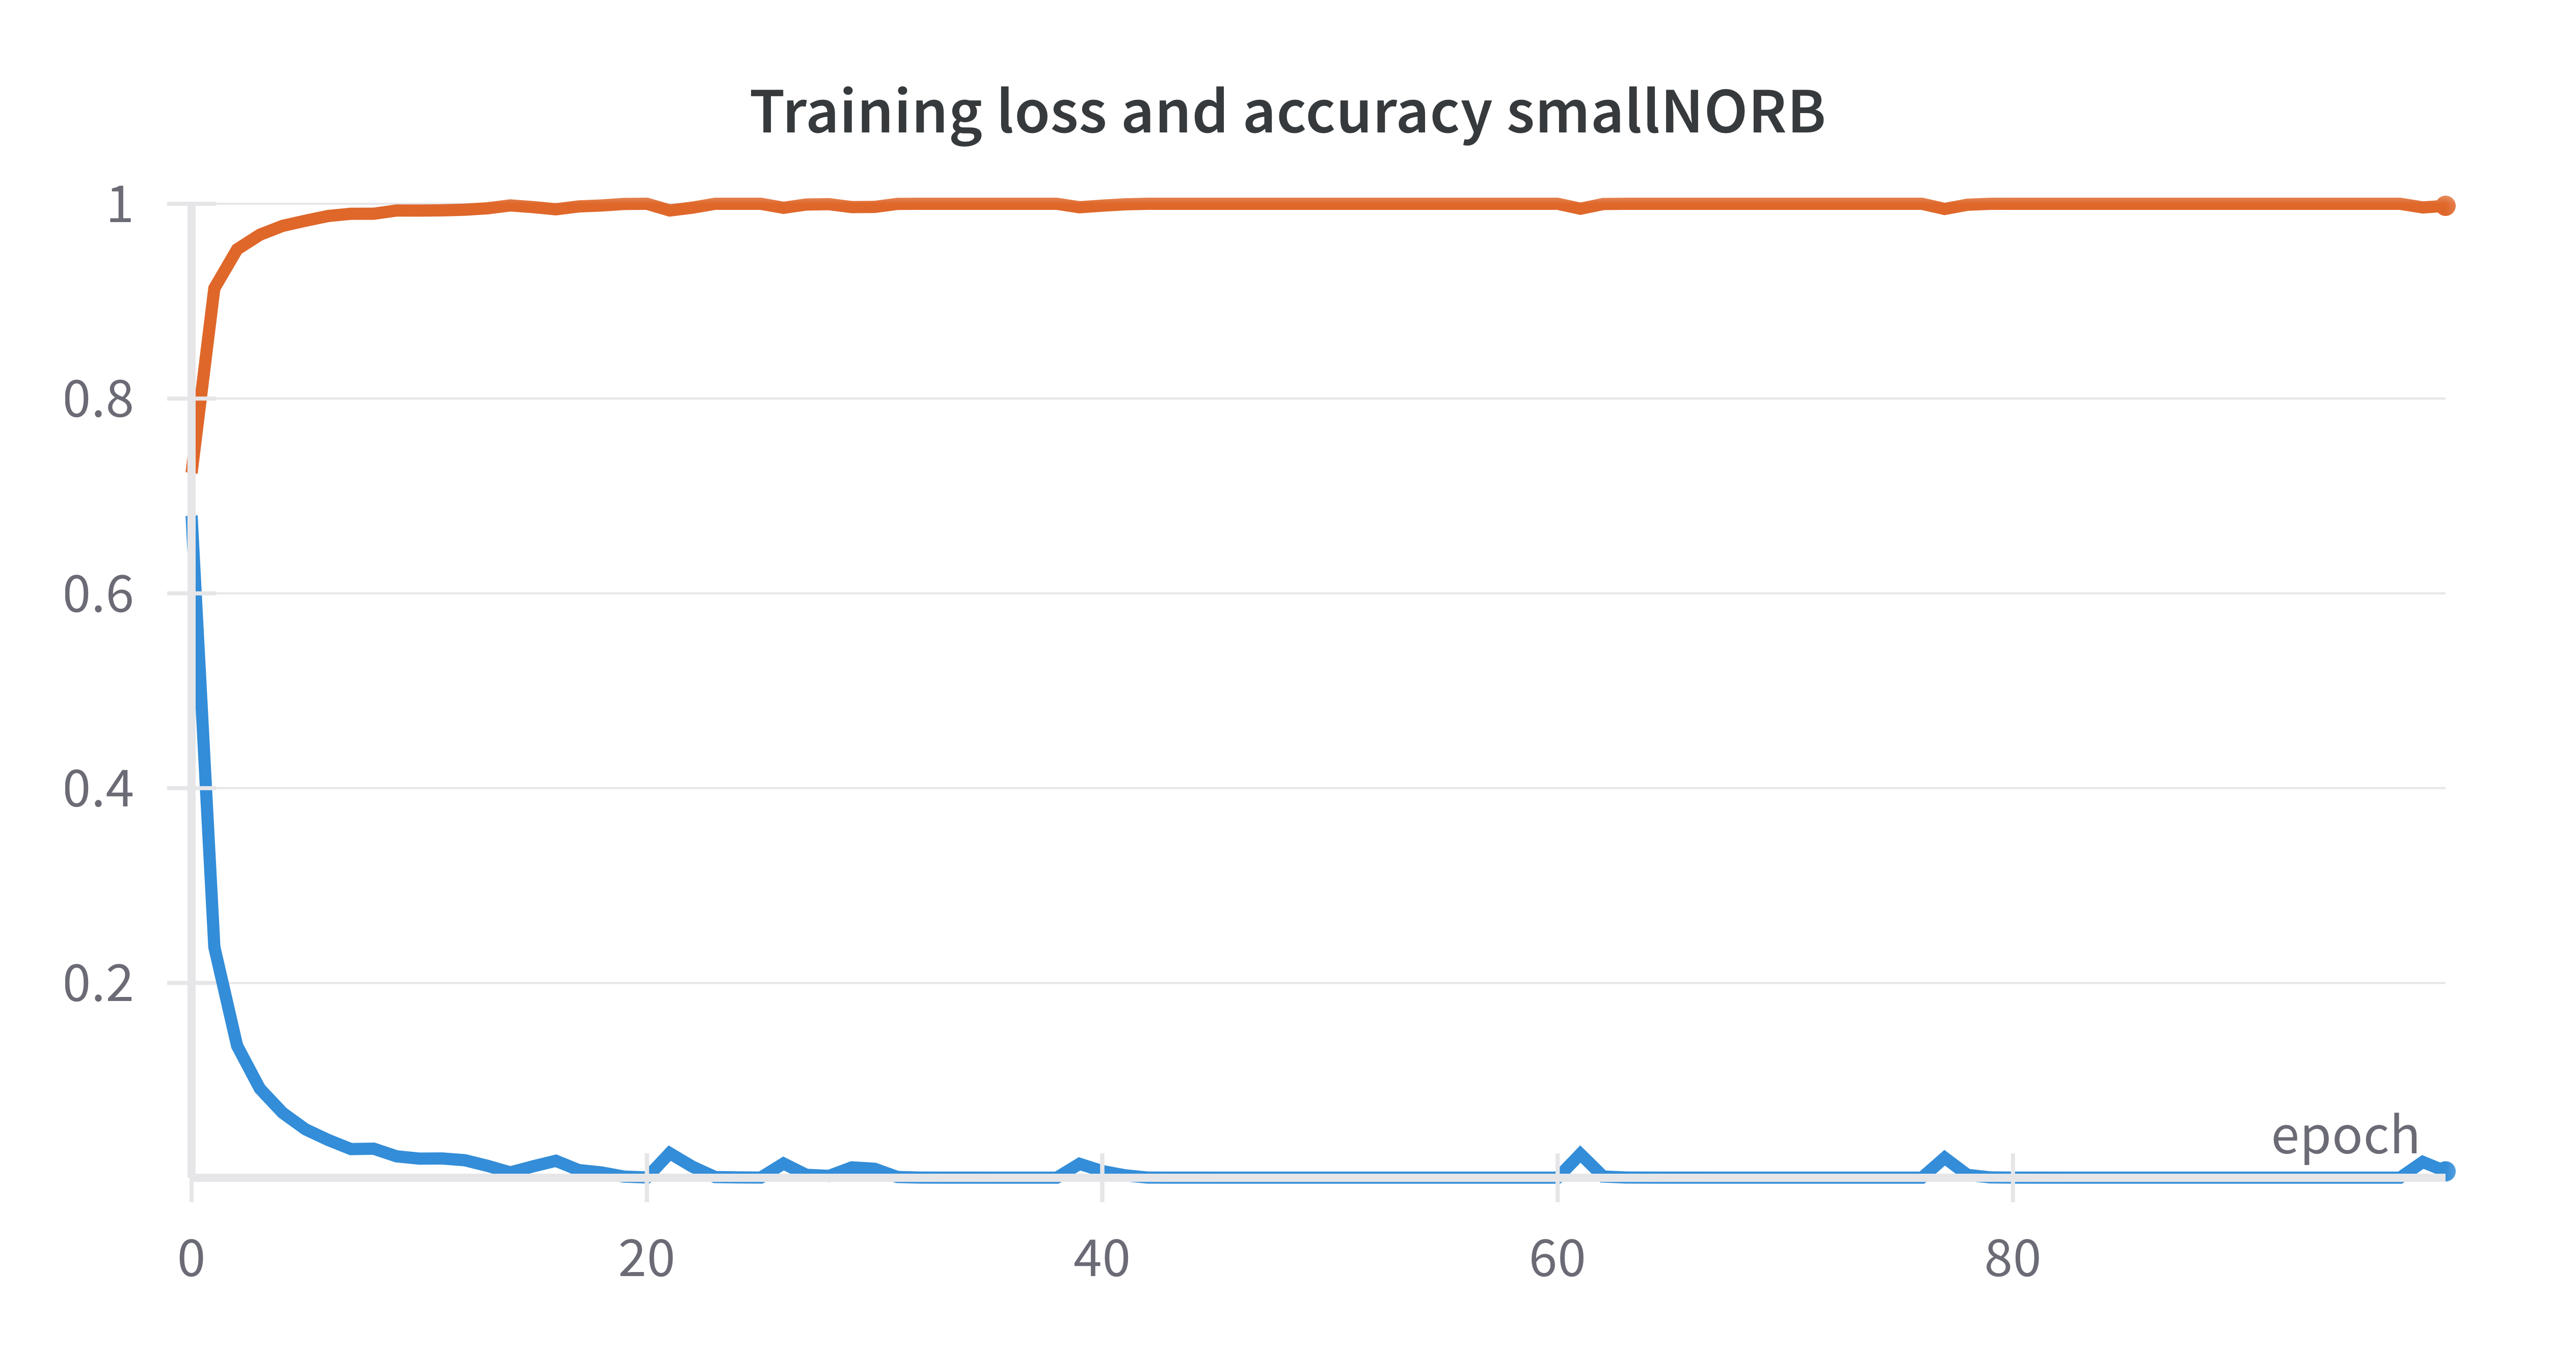
\includegraphics[width=1\linewidth]{smallnorb_train_loss_acc_mod.png}
		\caption{Training  loss/accuracy}
		\label{fig:smallnorb_train_loss_acc_mod}
	\end{subcaptionblock}%
	\begin{subcaptionblock}{.6\textwidth}
		\centering
		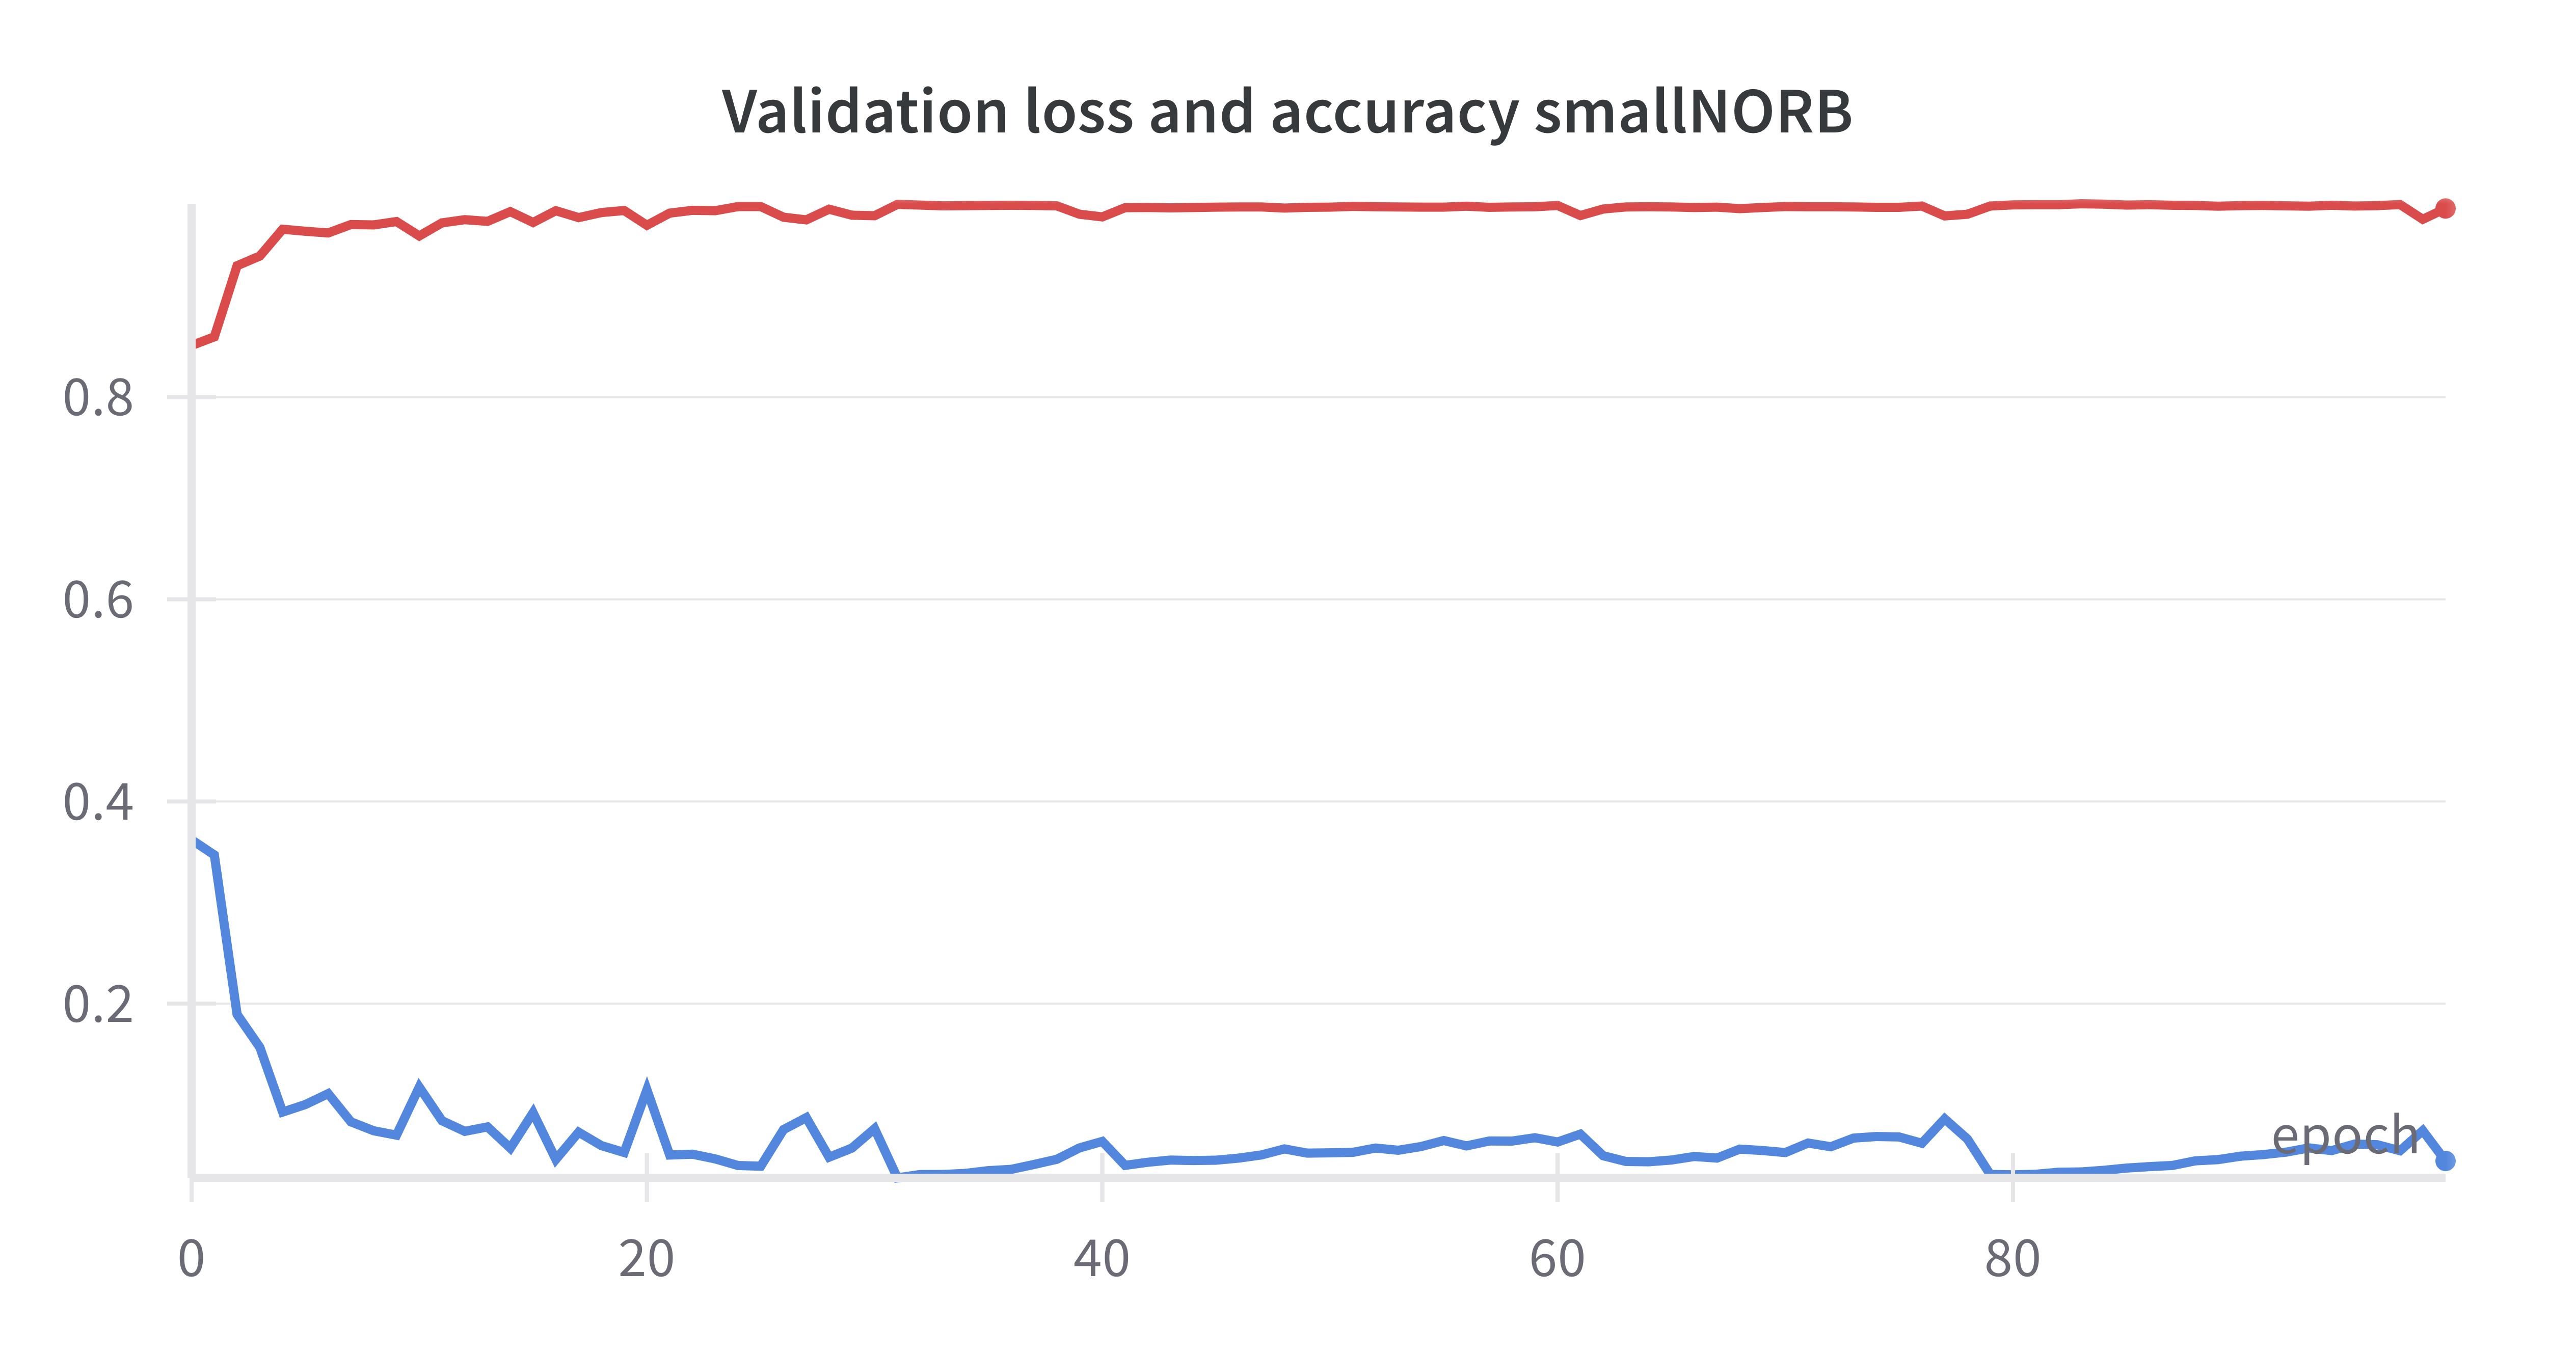
\includegraphics[width=1\linewidth]{smallnorb_val_loss_acc_mod.png}
		\caption{Validation loss/accuracy}
		\label{fig:smallnorb_val_loss_acc_mod}
	\end{subcaptionblock}%
	}
	\caption{Metriche del dataset smallNORB (con training set modificato)}
	\label{fig:smallnorb_train_val_loss_acc_mod}
\end{figure}

Nel codice degli autori, oltre alla diversa divisione del dataset, il modello non ha un layer di dropout e non è presente ne la funzione di \textit{fit}, ne la configurazione dell'\textit{early stopping}.

\subsubsection{Codice del progetto}
Nel codice del progetto il dataset smallNORB è suddiviso come descritto nell'articolo, cioè training set: 10800, validation set: 5400 e test set: 32400).
Il risultato ottenuto è quello della prima riga della tabella~\ref{tab:smallnorb_val_loss_acc_pt}.
\begin{table}[!ht]
	\centering
	\begin{tabular}[t]{|c|cc|}
		\hline
		& \textbf{Accuracy} & \textbf{Loss} \\
		\hline
		training set articolo& 0.718 & 2.001\\
		training set modificato& 0.849 & 0.445 \\
		articolo & 0.865 & - \\ 
		\hline
	\end{tabular}
	\caption{Test loss/accuracy smallNORB (con validation set)}
	\label{tab:smallnorb_val_loss_acc_pt}
\end{table}

\noindent Come prevedibile, anche in questo caso abbiamo un valore di loss molto elevato.
In figura~\ref{fig:smallnorb_train_val_loss_acc_original_pt} possiamo osservare la stessa curva anomale della validation loss, come visto in precedenza nel codice degli autori.
\begin{figure}[ht]
	\centerline{% center image to the page, not to text
		\begin{subcaptionblock}{.6\textwidth}
			\centering
			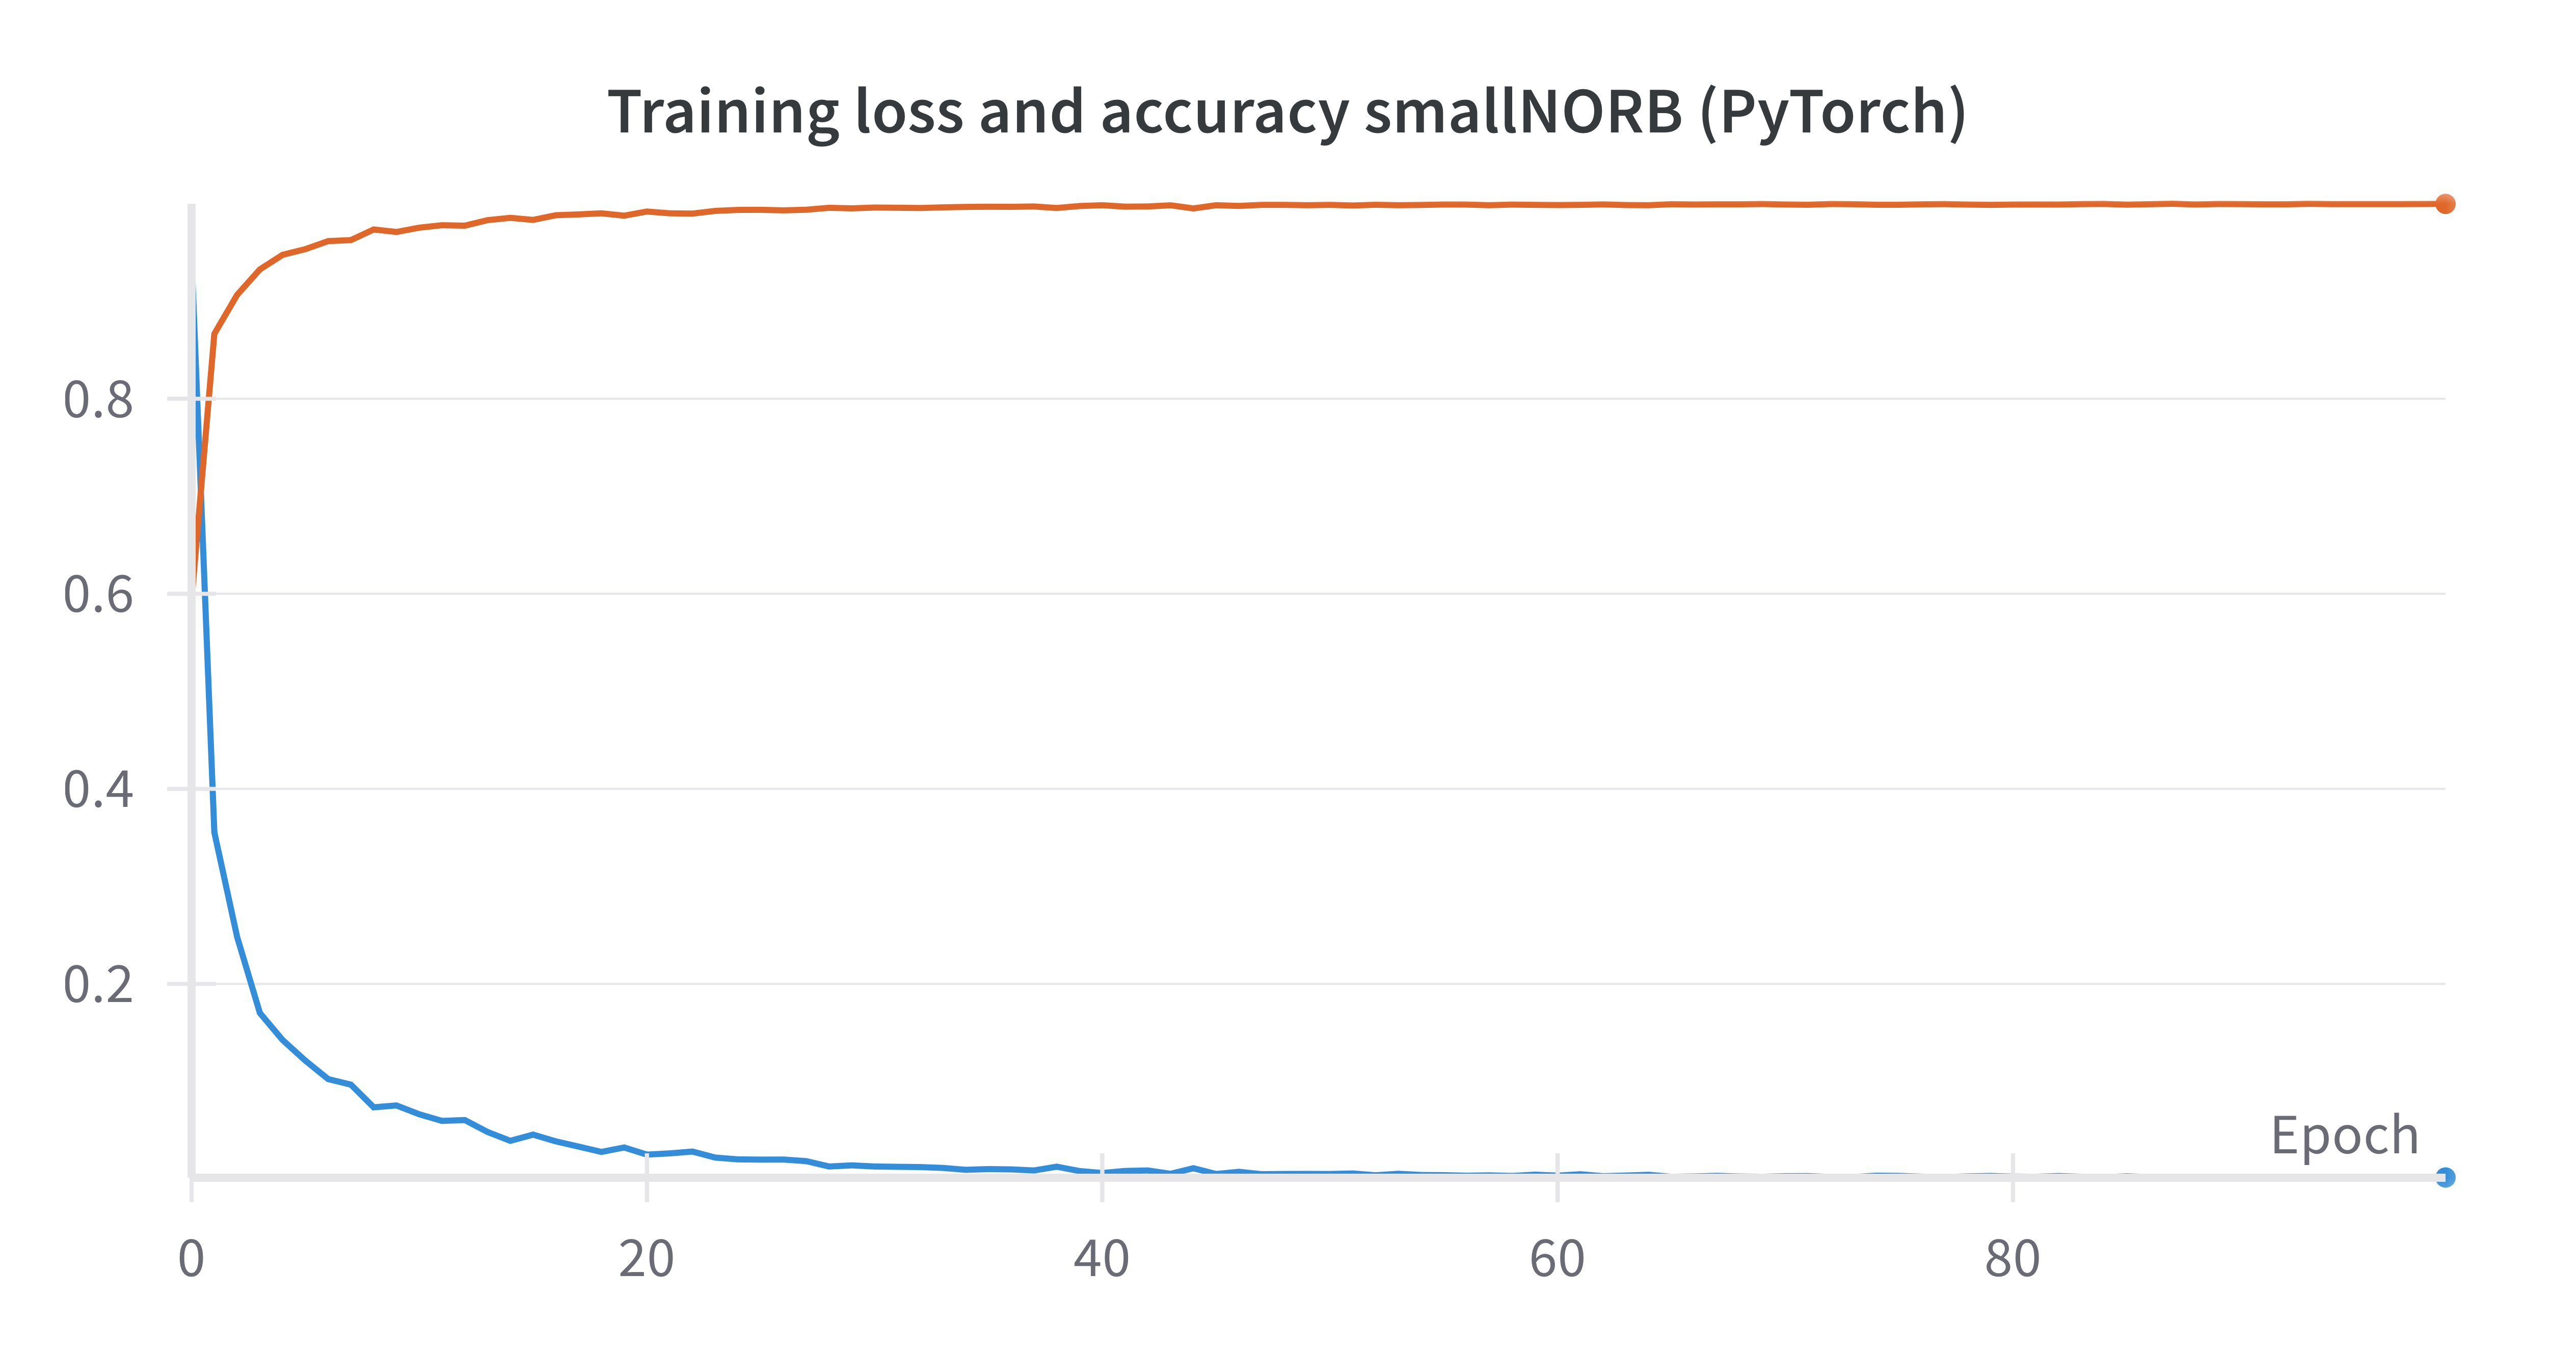
\includegraphics[width=1\linewidth]{smallnorb_train_loss_acc_original_pt.png}
			\caption{Training  loss/accuracy}
			\label{fig:smallnorb_train_loss_acc_original_pt}
		\end{subcaptionblock}%
		\begin{subcaptionblock}{.6\textwidth}
			\centering
			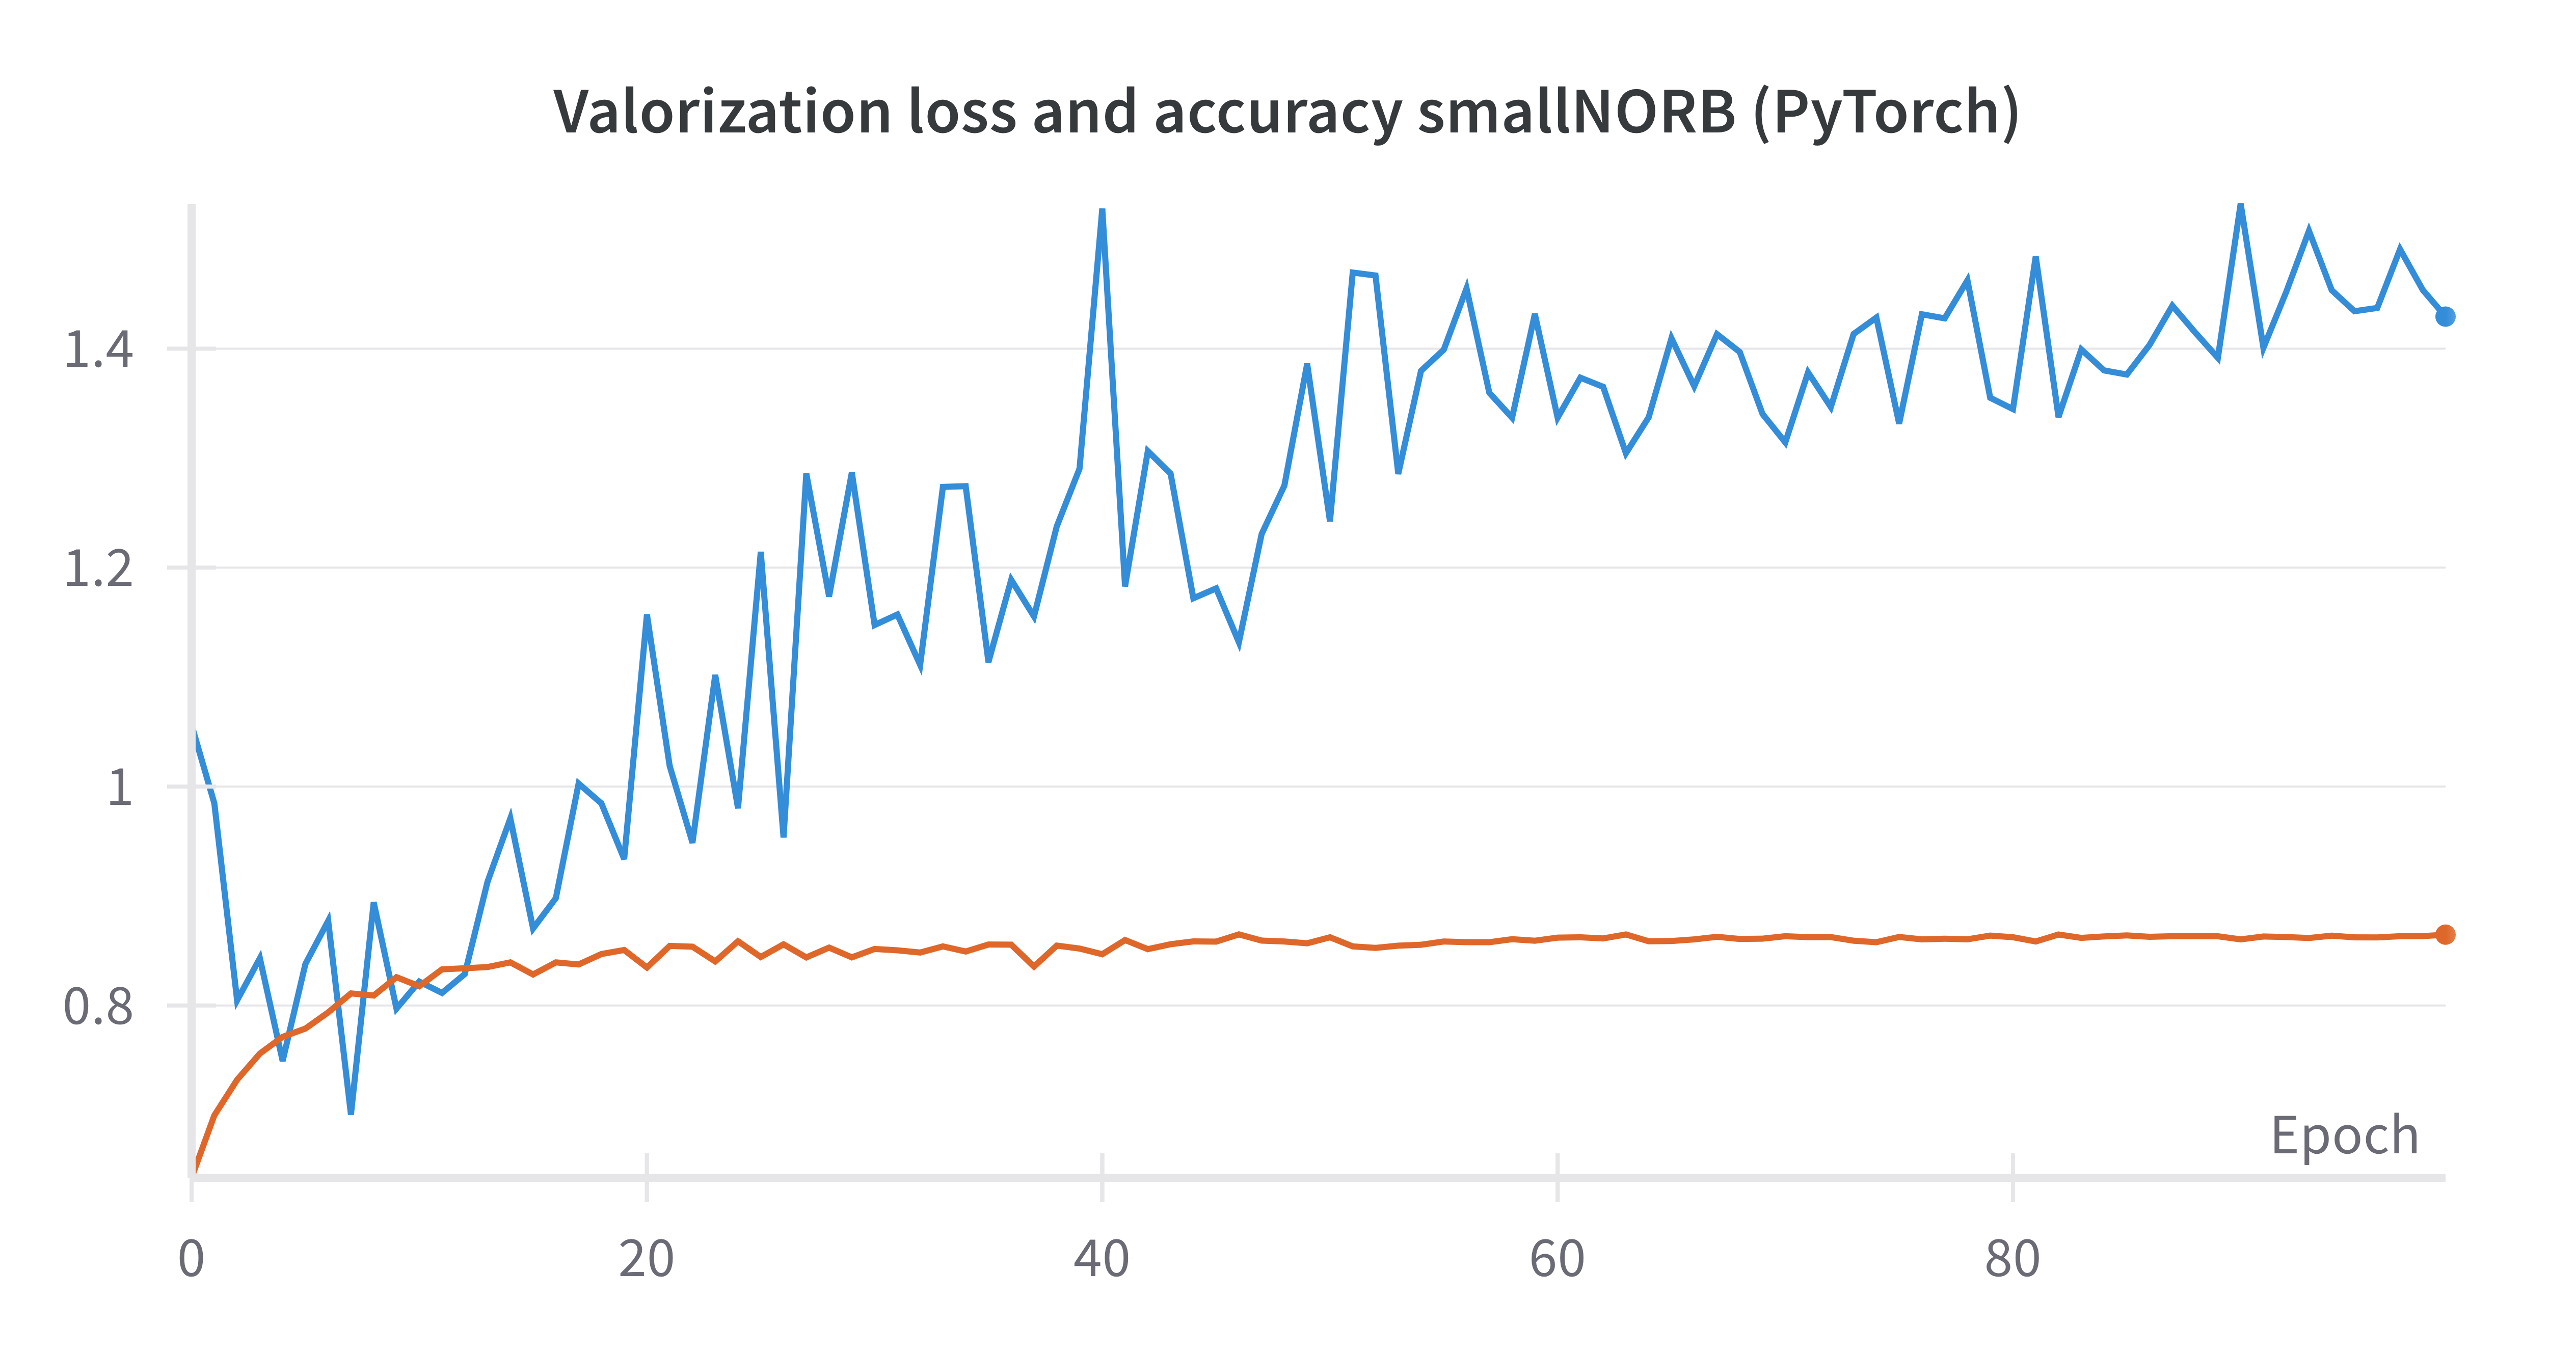
\includegraphics[width=1\linewidth]{smallnorb_val_loss_acc_original_pt.png}
			\caption{Validation loss/accuracy}
			\label{fig:smallnorb_val_loss_acc_original_pt}
		\end{subcaptionblock}%
	}
	\caption{Metriche del dataset smallNORB (con training set da articolo)}
	\label{fig:smallnorb_train_val_loss_acc_original_pt}
\end{figure}
Modificando il codice del progetto, aumentando i dati del training set a 21600 e riducendo quelli del test set a 21600, il modello sembra funzionare meglio, come possiamo vedere in figura~\ref{fig:smallnorb_train_val_loss_acc_mod_pt}.
I risultati ottenuti sono quelli presenti nella seconda riga della tabella~\ref{tab:smallnorb_val_loss_acc_pt}.

\begin{figure}[ht]
	\centerline{% center image to the page, not to text
		\begin{subcaptionblock}{.6\textwidth}
			\centering
			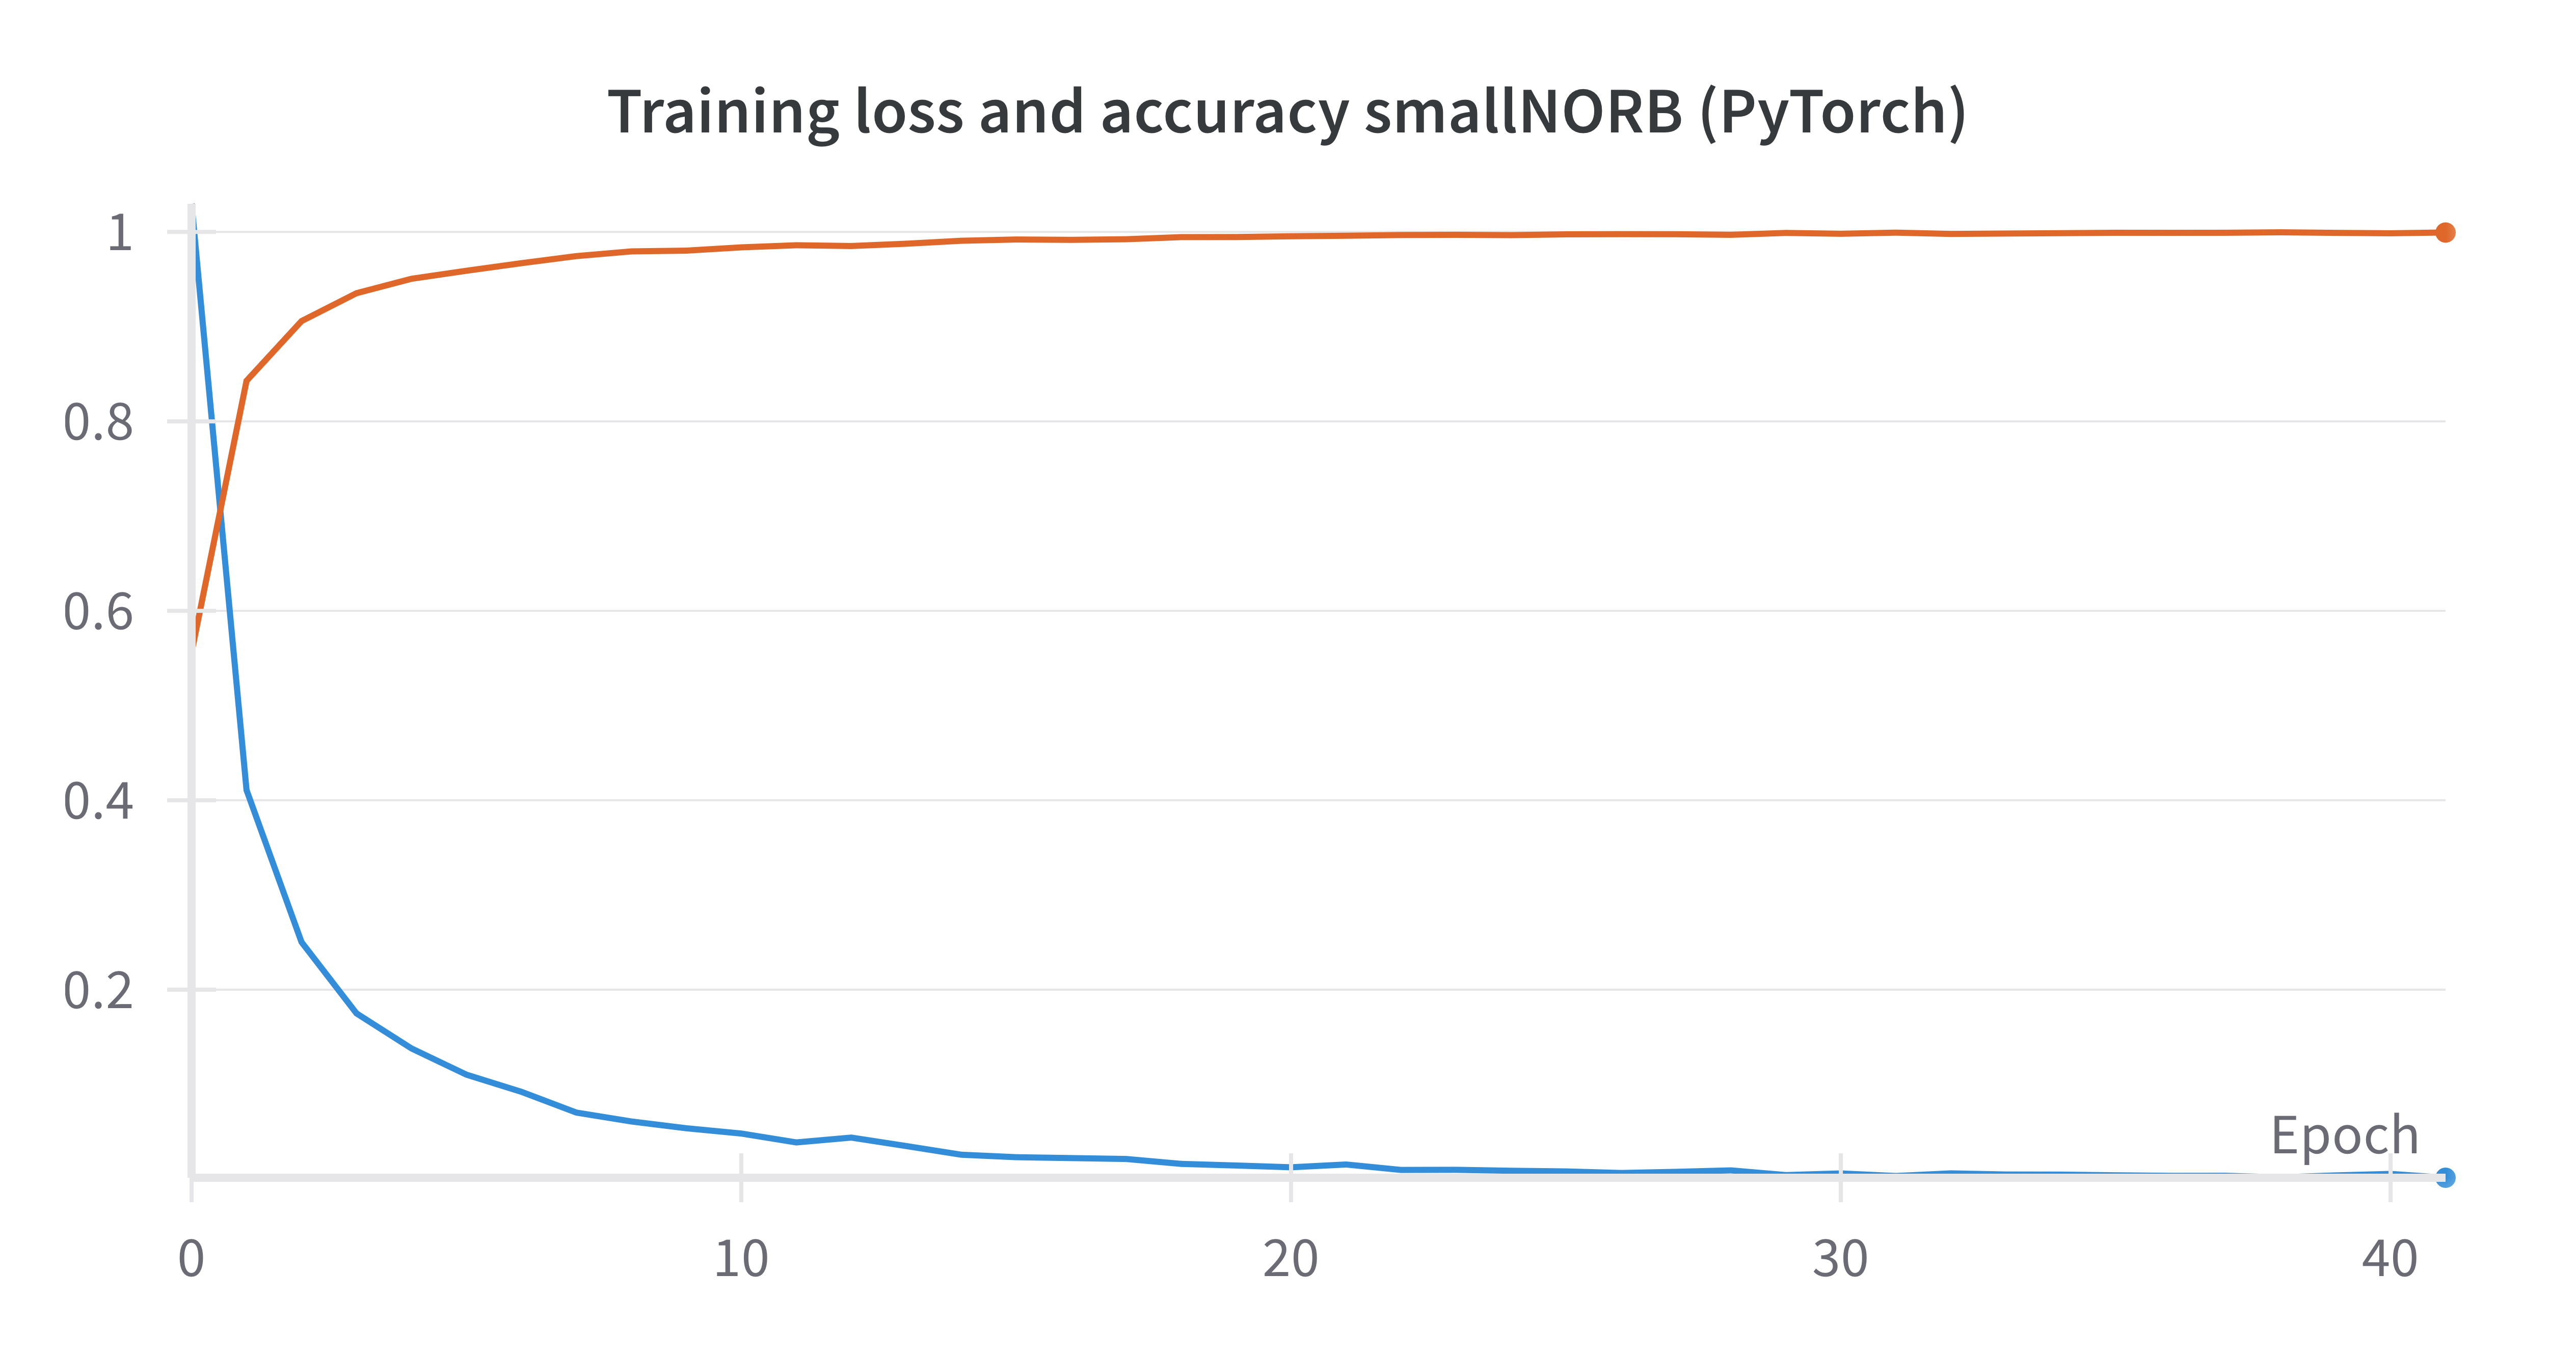
\includegraphics[width=1\linewidth]{smallnorb_train_loss_acc_mod_pt.png}
			\caption{Training  loss/accuracy}
			\label{fig:smallnorb_train_loss_acc_mod_pt.}
		\end{subcaptionblock}%
		\begin{subcaptionblock}{.6\textwidth}
			\centering
			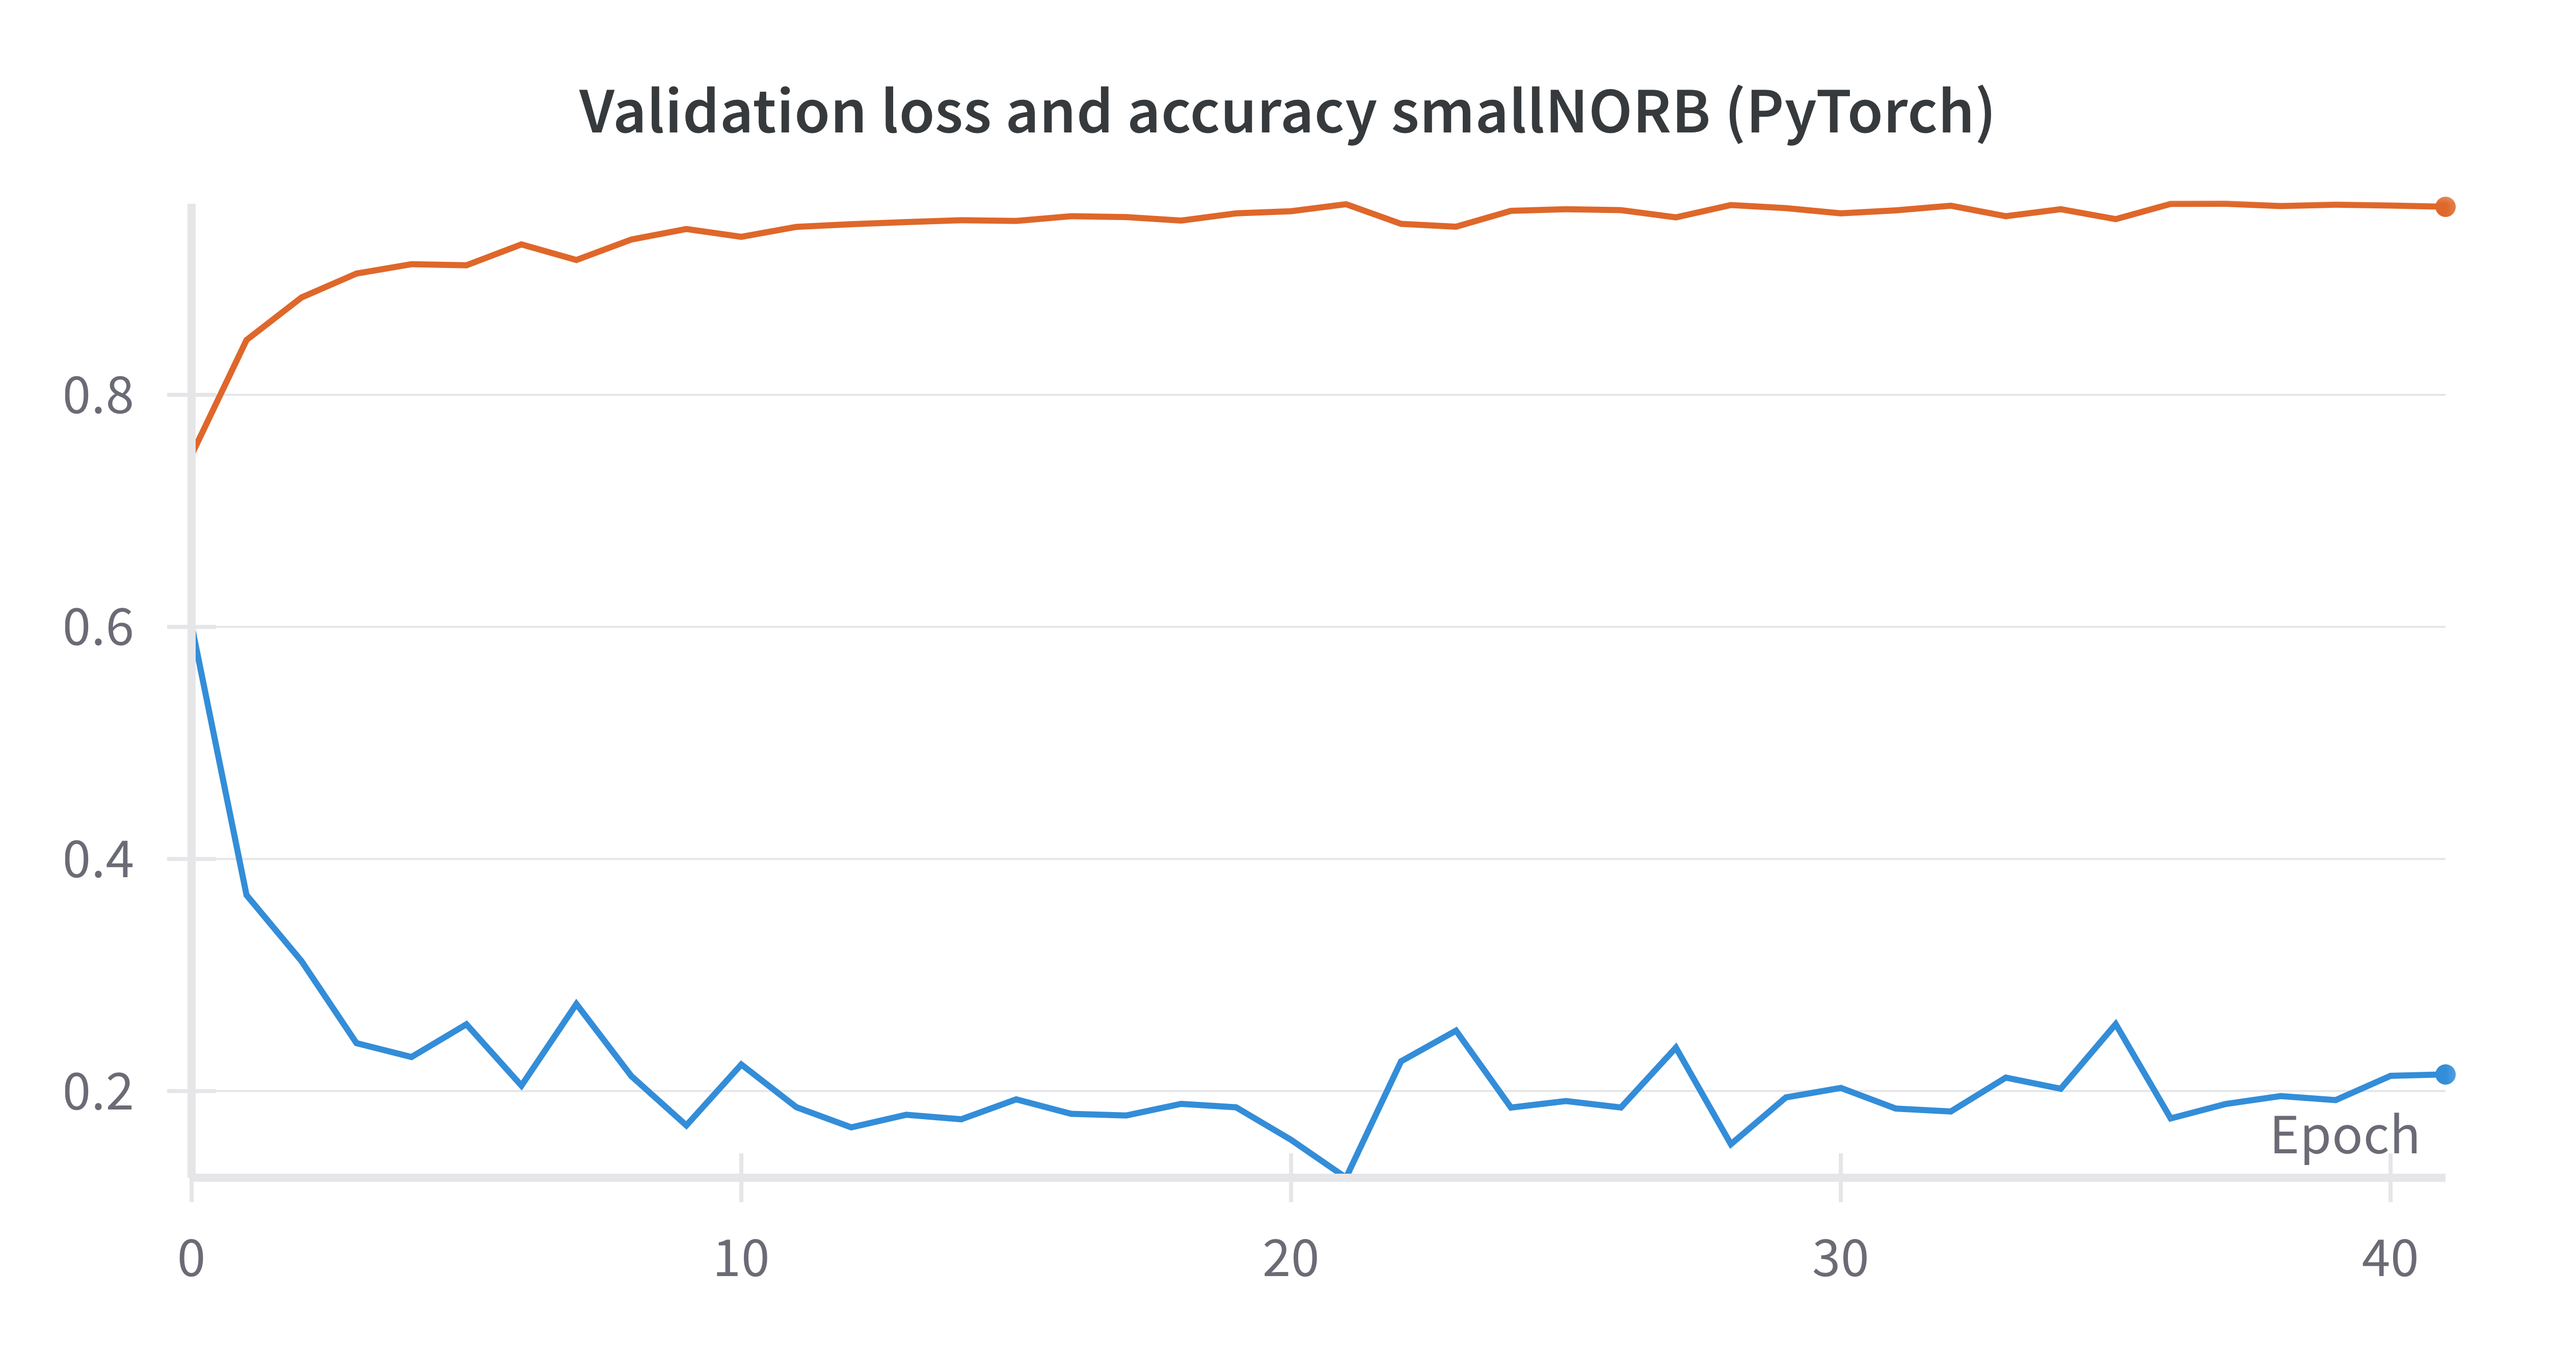
\includegraphics[width=1\linewidth]{smallnorb_val_loss_acc_mod_pt.png}
			\caption{Validation loss/accuracy}
			\label{fig:smallnorb_val_loss_acc_mod_pt.}
		\end{subcaptionblock}%
	}
	\caption{Metriche del dataset smallNORB (con training set modificato)}
	\label{fig:smallnorb_train_val_loss_acc_mod_pt}
\end{figure}


\subsection{ModelNet2D}

\subsubsection{Codice originale}
Visto che questo dataset non è composto da immagini binoculari, gli autori hanno dovuto utilizzare coppie di immagini con gradi di azimut successivi per simulare le immagini binoculari.
Quindi 10.800 coppie di immagini vengono utilizzate per il training set, 32.400 coppie per il test set e 5.400 coppie di immagini per il validation set.


\newpage

\section{Risultati e commenti}
%TODO Risultati e commenti
In questa esperienza di laboratorio abbiamo ricavato in modo empirico le costanti di taratura della funzione di trasferimento di un sensore di temperatura, realizzato con un termistore NTC.
Abbiamo inoltre confermato il fatto che questo tipo di sensori, vista la maggior massa dovuta ai loro rivestimenti protettivi, impiegano diverso tempo per raggiungere l'equilibrio termico.

\printbibliography[heading=bibintoc] %Prints bibliography

\end{document}
